\documentclass[final,oneside,onecolumn,12pt,a4paper]{book}%
%薛丞宏加的
\usepackage{fontspec} 
\usepackage{xeCJK} 
\XeTeXlinebreaklocale "zh" 
\XeTeXlinebreakskip = 0pt plus 1pt 
\pagestyle{empty}
%Select fonts
%\setmainfont[Mapping=tex-text]{Times New Roman} % rm
%\setsansfont[Mapping=tex-text]{Arial}           % sf
%\setmonofont{Courier New}                       % tt
\setCJKmainfont{DFKai-SB} %xelatex 標楷體
\setCJKmonofont{MingLiU}  %xelatex 細明體
\linespread{3}

\usepackage[toc,page]{appendix}%加附錄
\usepackage{makecell}%予表的第一格會當有一條舒舒的線隔做兩格
\usepackage{tablefootnote}%佇表內底用註解footnote in table
\usepackage{pgfplots}%畫圖表的套件

\usepackage{colortbl}
\usepackage{ruby}

\usepackage{graphicx}
%\usepackage[export]{adjustbox}

%\definecolor{intnull}{RGB}{213,229,255}

\renewcommand{\rubysep}{-4ex}

\makeatletter%予臺語音標會當佇字下跤
\newcommand{\rubybot}[2]{
  \@tempdimc \f@size\p@
  \begin{tabular}[t]{@{}>{\hspace{-6pt}}l<{\hspace{-9pt}}@{}}
%	\arrayrulecolor{red}\hline
%    #1\\[-1.7em]
	#1\\[-1.7em]
    \fontsize{.5\@tempdimc}{.5\@tempdimc}\selectfont%
    \setlength{\normalbaselineskip}{0pt}#2 
    %\cellcolor{intnull}
    
%	\\\arrayrulecolor{blue}\hline
  \end{tabular}%
}
\makeatother

%\fboxrule=4pt%border thickness

\usepackage{ifthen}

\newcommand{\too}[1]{\raisebox{-.2\height}{\includegraphics[height=1em]{#1}}}

\newcommand{\ji}[1]{\too{字/#1}}

\newcommand{\im}[1]{\too{音/#1}}
%\raisebox{-.2\height}{\includegraphics[height=1em]{音/#1}}

\newcommand{\tsoo}[3]{
\rubybot{#1\ifthenelse{\equal{#2}{}}{}{\im{#2}}}{#3}
}
%薛丞宏加的

\usepackage{amsmath}
\usepackage{amsfonts}
\usepackage{amssymb}
\usepackage{url}
\usepackage{hyperref}
\usepackage{algorithm}
\usepackage{algorithmic}
\usepackage{graphicx}%
\setcounter{MaxMatrixCols}{30}
\usepackage[left=3cm, right=2cm, top=2.5cm, bottom=2.5cm]{geometry}
%TCIDATA{OutputFilter=latex2.dll}
%TCIDATA{Version=5.50.0.2953}
%TCIDATA{Created=Monday, May 12, 2003 22:46:51}
%TCIDATA{LastRevised=Friday, August 30, 2013 14:39:59}
%TCIDATA{<META NAME="GraphicsSave" CONTENT="32">}
%TCIDATA{<META NAME="SaveForMode" CONTENT="1">}
%TCIDATA{BibliographyScheme=BibTeX}
%TCIDATA{<META NAME="DocumentShell" CONTENT="Standard LaTeX\Blank - Standard LaTeX Article">}
%TCIDATA{Language=American English}
%TCIDATA{PageSetup=72,72,72,72,0}
%TCIDATA{Counters=arabic,1}
%TCIDATA{AllPages=
%H=36
%F=36
%}
%BeginMSIPreambleData
\providecommand{\U}[1]{\protect\rule{.1in}{.1in}}
%EndMSIPreambleData
\oddsidemargin 0.0in
\textheight=8.5in
\textwidth=6.5in
\headheight=0.0in
\topmargin=0.0in
\newtheorem{theorem}{Theorem}
\newtheorem{abstract}{abstract}
\newtheorem{acknowledgement}[theorem]{Acknowledgement}
\newtheorem{axiom}[theorem]{Axiom}
\newtheorem{case}[theorem]{Case}
\newtheorem{claim}[theorem]{Claim}
\newtheorem{conclusion}[theorem]{Conclusion}
\newtheorem{condition}[theorem]{Condition}
\newtheorem{conjecture}[theorem]{Conjecture}
\newtheorem{corollary}[theorem]{Corollary}
\newtheorem{criterion}[theorem]{Criterion}
\newtheorem{definition}[theorem]{Definition}
\newtheorem{example}[theorem]{Example}
\newtheorem{exercise}[theorem]{Exercise}
\newtheorem{lemma}[theorem]{Lemma}
\newtheorem{notation}[theorem]{Notation}
\newtheorem{problem}[theorem]{Problem}
\newtheorem{proposition}[theorem]{Proposition}
\newtheorem{remark}[theorem]{Remark}
\newtheorem{solution}[theorem]{Solution}
\newtheorem{summary}[theorem]{Summary}
\interdisplaylinepenalty=2500
\sloppy
\pagenumbering{arabic}
\pagestyle{plain}
\renewcommand{\baselinestretch}{2}
\begin{document}
\begin{titlepage}

\begin{center}

   

\textsc{\Huge 國 立 交 通 大 學} %38
\\[2em]
\textsc{\LARGE 資訊科學與工程研究所} %28
\\[2em]
\textsc{\LARGE 碩 士 論 文} %28
\\[3em]

% Title
{\huge \bfseries 漢語間統計式機器翻譯語料處理-用臺灣閩南語示範 } %20
\\[1em]
{\LARGE Corpus Preprocessing for Statistical Machine Translation between the Chinese Languages Using Taiwan Southern Min as Examples}
\\[3em]

\begin{table}[H]
\centering
\Large
\begin{tabular}{ll}
研 究 生: & 薛丞宏\\ %18
指導教授: & 張智星教授\\ %18
 & 易志偉教授\\ %18
\end{tabular}
\end{table}

\vfill

{\large 中 華 民 國  103  年  11  月}

\end{center}

\end{titlepage}


\frontmatter
\chapter{踏話頭}
\tsoo{臺}{⿳⿳ㄉㄞˊ}{tâi}
\tsoo{灣}{⿳⿳ㄨㄢˊ}{uân}
\tsoo{是}{⿳⿳ㄒㄧ˫}{sī}
\tsoo{一}{⿳⿳⿳ㄐㄧ㆐ㆵ}{tsi̍t}
\tsoo{个}{⿳ㆤˊ}{ê}
\tsoo{多}{⿳ㄉㄜ}{to}
\tsoo{元}{⿳⿳⿳ㆣㄨㄢˊ}{guân}
\tsoo{民}{⿳⿳⿳ㆠㄧㄣˊ}{bîn}
\tsoo{族}{⿳⿳⿳ㄗㆦ㆐ㆶ}{tso̍k}
\tsoo{、}{}{、}
\tsoo{多}{⿳ㄉㄜ}{to}
\tsoo{元}{⿳⿳⿳ㆣㄨㄢˊ}{guân}
\tsoo{語}{⿳⿳ㆣㄨˋ}{gú}
\tsoo{言}{⿳⿳ㆣㄢˊ}{gân}
\tsoo{的}{⿳ㆤˊ}{ê}
\tsoo{國}{⿳⿳ㄍㆦㆶ}{kok}
\tsoo{家}{⿳ㄍㄚ}{ka}
\tsoo{,}{}{,}
\tsoo{講}{⿳⿳ㄍㆲˋ}{kóng}
\tsoo{母}{⿳⿳ㆠㄨˋ}{bú}
\tsoo{語}{⿳⿳ㆣㄨˋ}{gú}
\tsoo{、}{}{、}
\tsoo{使}{⿳⿳ㄙㄨˋ}{sú}
\tsoo{用}{⿳⿳ㄧㆲ˫}{iōng}
\tsoo{母}{⿳⿳ㆠㄨˋ}{bú}
\tsoo{語}{⿳⿳ㆣㄨˋ}{gú}
\tsoo{嘛}{⿳⿳ㄇㄚ˫}{mā}
\tsoo{是}{⿳⿳ㄒㄧ˫}{sī}
\tsoo{人}{⿳⿳ㄌㄤˊ}{lâng}
\tsoo{上}{⿳⿳⿳ㄒㄧㆲ˫}{siōng}
\tsoo{基}{⿳ㄍㄧ}{ki}
\tsoo{本}{⿳⿳⿳ㄅㄨㄣˋ}{pún}
\tsoo{的}{⿳ㆤˊ}{ê}
\tsoo{權}{⿳⿳⿳ㄎㄨㄢˊ}{khuân}
\tsoo{利}{⿳⿳ㄌㄧ˫}{lī}
\tsoo{,}{}{,}
\tsoo{毋}{⿳ㆬ˫}{m̄}
\tsoo{過}{⿳⿳ㄍㄨ˪}{kù}
\tsoo{母}{⿳⿳ㆠㄨˋ}{bú}
\tsoo{語}{⿳⿳ㆣㄨˋ}{gú}
\tsoo{的}{⿳ㆤˊ}{ê}
\tsoo{相}{⿳⿳ㄒㄧㆲ}{siong}
\tsoo{關}{⿳⿳ㄍㄨㄢ}{kuan}
\tsoo{應}{⿳⿳ㄧㄥ˪}{ìng}
\tsoo{用}{⿳⿳ㄧㆲ˫}{iōng}
\tsoo{煞}{⿳⿳ㄙㆩㆷ}{sannh}
\tsoo{誠}{⿳⿳⿳ㄐㄧㆩˊ}{tsiânn}
\tsoo{少}{⿳⿳⿳ㄐㄧㄛˋ}{tsiór}
\tsoo{。}{}{.}
\tsoo{臺}{⿳⿳ㄉㄞˊ}{tâi}
\tsoo{灣}{⿳⿳ㄨㄢˊ}{uân}
\tsoo{本}{⿳⿳⿳ㄅㄨㄣˋ}{pún}
\tsoo{土}{⿳⿳ㄊㆦˋ}{thóo}
\tsoo{語}{⿳⿳ㆣㄨˋ}{gú}
\tsoo{言}{⿳⿳⿳ㆣㄧㄢˊ}{giân}
\tsoo{百}{⿳⿳ㄅㄚㆷ}{pah}
\tsoo{百}{⿳⿳ㄅㄚㆷ}{pah}
\tsoo{種}{⿳⿳⿳ㄐㄧㄥˋ}{tsíng}
\tsoo{,}{}{,}
\tsoo{本}{⿳⿳ㄅㆭˋ}{pńg}
\tsoo{論}{⿳⿳⿳ㄌㄨㄣ˫}{lūn}
\tsoo{文}{⿳⿳⿳ㆠㄨㄣˊ}{bûn}
\tsoo{先}{⿳⿳ㄒㄧㄥ}{sing}
\tsoo{針}{⿳⿳ㄐㄧㆰ}{tsiam}
\tsoo{對}{⿳⿳⿳ㄉㄨㄧ˪}{tuì}
\tsoo{閩}{⿳⿳ㆠㄢˊ}{bân}
\tsoo{南}{⿳⿳ㄌㆰˊ}{lâm}
\tsoo{語}{⿳⿳ㆣㆨˋ}{gír}
\tsoo{,}{}{,}
\tsoo{研}{⿳⿳⿳ㆣㄧㄢˋ}{gián}
\tsoo{究}{⿳⿳⿳ㄍㄧㄨ˪}{kiù}
\tsoo{伊}{⿳ㄧ }{i}
\tsoo{翻}{⿳⿳ㄏㄨㄢ}{huan}
\tsoo{譯}{⿳⿳ㄧ㆐ㆶ}{i̍k}
\tsoo{語}{⿳⿳ㆣㆨˋ}{gír}
\tsoo{料}{⿳⿳⿳ㄌㄧㄠ˫}{liāu}
\tsoo{的}{⿳ㆤˊ}{ê}
\tsoo{特}{⿳⿳⿳ㄉㄧ㆐ㆶ}{ti̍k}
\tsoo{性}{⿳⿳⿳ㄒㄧㄥ˪}{sìng}
\tsoo{,}{}{,}
\tsoo{希}{⿳ㄏㄧ}{hi}
\tsoo{望}{⿳⿳ㆠㄤ˫}{bāng}
\tsoo{除}{⿳⿳ㄉㄧˊ}{tî}
\tsoo{了}{⿳⿳⿳ㄌㄧㄠˋ}{liáu}
\tsoo{閩}{⿳⿳ㆠㄢˊ}{bân}
\tsoo{南}{⿳⿳ㄌㆰˊ}{lâm}
\tsoo{語}{⿳⿳ㆣㆨˋ}{gír}
\tsoo{本}{⿳⿳⿳ㄅㄨㄣˋ}{pún}
\tsoo{身}{⿳⿳ㄒㄧㄣ}{sin}
\tsoo{以}{⿳ㄧˋ}{í}
\tsoo{外}{⿳⿳⿳ㆣㄨㄚ˫}{guā}
\tsoo{,}{}{,}
\tsoo{嘛}{⿳⿳ㄇㄚ˫}{mā}
\tsoo{希}{⿳ㄏㄧ}{hi}
\tsoo{望}{⿳⿳ㆠㄤ˫}{bāng}
\tsoo{研}{⿳⿳⿳ㆣㄧㄢˋ}{gián}
\tsoo{究}{⿳⿳⿳ㄍㄧㄨ˪}{kiù}
\tsoo{結}{⿳⿳⿳ㄍㄧㄚㆵ}{kiat}
\tsoo{果}{⿳⿳ㄍㄜˋ}{kó}
\tsoo{對}{⿳⿳⿳ㄉㄨㄧ˪}{tuì}
\tsoo{別}{⿳⿳⿳ㄅㄧㄚㆵ}{piat}
\tsoo{的}{⿳⿳⿳ㄉㄧ㆐ㆶ}{ti̍k}
\tsoo{本}{⿳⿳⿳ㄅㄨㄣˋ}{pún}
\tsoo{土}{⿳⿳ㄊㆦˋ}{thóo}
\tsoo{語}{⿳⿳ㆣㄨˋ}{gú}
\tsoo{言}{⿳⿳⿳ㆣㄧㄢˊ}{giân}
\tsoo{有}{⿳ㄨ˫}{ǔ}
\tsoo{幫}{⿳ㄅㄤ}{pang}
\tsoo{助}{⿳⿳ㄗㆦ˫}{tsōo}
\tsoo{。}{}{.}


\tsoo{本}{⿳⿳ㄅㆭˋ}{pńg}
\tsoo{論}{⿳⿳⿳ㄌㄨㄣ˫}{lūn}
\tsoo{文}{⿳⿳⿳ㆠㄨㄣˊ}{bûn}
\tsoo{主}{⿳⿳ㄗㄨˋ}{tsú}
\tsoo{要}{⿳⿳ㄧㄠ˪}{iàu}
\tsoo{有}{⿳ㄨ˫}{ū}
\tsoo{四}{⿳⿳ㄒㄧ˪}{sì}
\tsoo{个}{⿳ㆤˊ}{ê}
\tsoo{貢}{⿳⿳ㄍㆲ˪}{kòng}
\tsoo{獻}{⿳⿳⿳ㄏㄧㄢ˪}{hiàn}
\tsoo{。}{}{.}
\tsoo{第}{⿳⿳ㄉㆤ˫}{tē}
\tsoo{一}{⿳⿳⿳ㄐㄧ㆐ㆵ}{tsi̍t}
\tsoo{个}{⿳ㆤˊ}{ê}
\tsoo{是}{⿳⿳ㄒㄧ˫}{sī}
\tsoo{本}{⿳⿳ㄅㆭˋ}{pńg}
\tsoo{論}{⿳⿳⿳ㄌㄨㄣ˫}{lūn}
\tsoo{文}{⿳⿳⿳ㆠㄨㄣˊ}{bûn}
\tsoo{提}{⿳⿳⿳ㄊㆤ㆐ㆷ}{the̍h}
\tsoo{出}{⿳⿳ㄘㄨㆵ}{tshut}
\tsoo{「}{}{“}
\tsoo{拄}{⿳⿳ㄉㄨˋ}{tú}
\tsoo{好}{⿳⿳ㄏㄜˋ}{hó}
\tsoo{長}{⿳⿳ㄉㆭˊ}{tn̂g}
\tsoo{度}{⿳⿳ㄉㆦ˫}{tōo}
\tsoo{斷}{⿳⿳⿳ㄉㄨㆪ˫}{tuīnn}
\tsoo{詞}{⿳⿳ㄙㄨˊ}{sû}
\tsoo{」}{}{”}
\tsoo{的}{⿳˙ㆤ}{0ê}
\tsoo{演}{⿳⿳ㄧㄢˋ}{ián}
\tsoo{算}{⿳⿳ㄙㆭ˪}{sǹg}
\tsoo{法}{⿳⿳⿳ㄏㄨㄚㆵ}{huat}
\tsoo{,}{}{,}
\tsoo{雖}{⿳⿳ㄙㄨㄧ}{sui}
\tsoo{然}{⿳⿳⿳ㄌㄧㄢˊ}{liân}
\tsoo{有}{⿳ㄨ˫}{ǔ}
\tsoo{改}{⿳⿳ㄍㄞˋ}{kái}
\tsoo{善}{⿳⿳⿳ㄒㄧㄢ˫}{siān}
\tsoo{「}{}{“}
\tsoo{長}{⿳⿳⿳ㄉㄧㆲ˪}{tiòng}
\tsoo{詞}{⿳⿳ㄙㄨˊ}{sû}
\tsoo{優}{⿳ㄧㄨ}{iu}
\tsoo{先}{⿳⿳ㄒㄧㄢ}{sian}
\tsoo{」}{}{”}
\tsoo{的}{⿳ㆤˊ}{ê}
\tsoo{缺}{⿳⿳⿳ㄎㄨㄚㆵ}{khuat}
\tsoo{點}{⿳⿳⿳ㄉㄧㆰˋ}{tiám}
\tsoo{,}{}{,}
\tsoo{毋}{⿳ㆬ˫}{m̄}
\tsoo{過}{⿳⿳ㄍㄨ˪}{kù}
\tsoo{效}{⿳⿳ㄏㄠ˫}{hāu}
\tsoo{果}{⿳⿳ㄍㄜˋ}{kó}
\tsoo{無}{⿳⿳ㆠㄜˊ}{bô}
\tsoo{明}{⿳⿳⿳ㆠㄧㄥˊ}{bîng}
\tsoo{顯}{⿳⿳⿳ㄏㄧㄢˋ}{hián}
\tsoo{,}{}{,}
\tsoo{正}{⿳⿳⿳ㄐㄧㄥ˪}{tsìng}
\tsoo{確}{⿳⿳ㄎㄚㆶ}{khak}
\tsoo{率}{⿳⿳ㄙㄨㆵ}{sut}
\tsoo{差}{⿳ㄘㆤ}{tshe}
\tsoo{無}{⿳⿳˙ㆠㄜ}{0bô}
$1\%$\tsoo{。}{}{,}
\tsoo{第}{⿳⿳ㄉㆤ˫}{tē}
\tsoo{二}{⿳⿳ㆢㄧ˫}{jī}
\tsoo{个}{⿳ㆤˊ}{ê}
\tsoo{貢}{⿳⿳ㄍㆲ˪}{kòng}
\tsoo{獻}{⿳⿳⿳ㄏㄧㄢ˪}{hiàn}
\tsoo{是}{⿳⿳ㄒㄧ˫}{sī}
\tsoo{漢}{⿳⿳ㄏㄢ˪}{hàn}
\tsoo{語}{⿳⿳ㆣㄧˋ}{gí}
\tsoo{語}{⿳⿳ㆣㄧˋ}{gí}
\tsoo{料}{⿳⿳⿳ㄌㄧㄠ˫}{liāu}
\tsoo{用}{⿳⿳ㄧㆲ˫}{iōng}
\tsoo{詞}{⿳⿳ㄙㄨˊ}{sû}
\tsoo{做}{⿳⿳⿳ㄗㄨㆤ˪}{tsuè}
\tsoo{單}{⿳ㄉㄢ}{tan}
\tsoo{位}{⿳⿳ㄨㄧ˫}{uī}
\tsoo{去}{⿳⿳˙ㄎㄧ}{0khì}
\tsoo{翻}{⿳⿳ㄏㄨㄢ}{huan}
\tsoo{譯}{⿳⿳ㄧ㆐ㆶ}{i̍k}
\tsoo{的}{⿳ㆤˊ}{ê}
\tsoo{時}{⿳⿳ㄒㄧˊ}{sî}
\tsoo{,}{}{,}
\tsoo{用}{⿳⿳ㄧㄥ˫}{īng}
\tsoo{斷}{⿳⿳⿳ㄉㄨㆪ˫}{tuīnn}
\tsoo{字}{⿳⿳ㄌㄧ˫}{lǐ}
\tsoo{翻}{⿳⿳ㄏㄨㄢ}{huan}
\tsoo{譯}{⿳⿳ㄧ㆐ㆶ}{i̍k}
\tsoo{會}{⿳⿳ㄮㆤ˫}{erē}
\tsoo{當}{⿳⿳ㄉㄤ˪}{tàng}
\tsoo{解}{⿳⿳ㄍㄞˋ}{kái}
\tsoo{決}{⿳⿳⿳ㄍㄨㄚㆵ}{kuat}
\tsoo{未}{⿳⿳ㆠㄧ˫}{bī}
\tsoo{知}{⿳ㄉㄧ}{ti}
\tsoo{詞}{⿳⿳ㄙㄨˊ}{sû}
\tsoo{問}{⿳⿳⿳ㆠㄨㄣ˫}{būn}
\tsoo{題}{⿳⿳ㄉㆤˊ}{tê}
\tsoo{,}{}{,}
\tsoo{會}{⿳⿳ㄮㆤ˫}{erē}
\tsoo{當}{⿳⿳ㄉㄤ˪}{tàng}
\tsoo{對}{⿳⿳⿳ㄉㄨㄧ˪}{tuì}
\tsoo{BLEU}{}{}
\tsoo{分}{⿳⿳ㄏㄨㄣ}{hun}
\tsoo{數}{⿳⿳ㄙㆦ˪}{sòo}
29.22
\tsoo{鈕}{⿳⿳⿳ㄌㄧㄨˋ}{liú}
\tsoo{到}{⿳⿳⿳ㄍㄚ㆐ㆷ}{ka̍h}
30.92
\tsoo{。}{}{.}
\tsoo{第}{⿳⿳ㄉㆤ˫}{tē}
\tsoo{三}{⿳ㄙㆩ}{sann}
\tsoo{个}{⿳ㆤˊ}{ê}
\tsoo{是}{⿳⿳ㄒㄧ˫}{sī}
\tsoo{提}{⿳⿳⿳ㄊㆤ㆐ㆷ}{the̍h}
\tsoo{出}{⿳⿳ㄘㄨㆵ}{tshut}
\tsoo{一}{⿳⿳⿳ㄐㄧ㆐ㆵ}{tsi̍t}
\tsoo{个}{⿳ㆤˊ}{ê}
\tsoo{自}{⿳⿳ㄗㄨ˫}{tsū}
\tsoo{動}{⿳⿳ㄉㆲ˫}{tōng}
\tsoo{整}{⿳⿳⿳ㄐㄧㄥˋ}{tsíng}
\tsoo{理}{⿳⿳ㄌㄧˋ}{lí}
\tsoo{漢}{⿳⿳ㄏㄢ˪}{hàn}
\tsoo{語}{⿳⿳ㆣㄧˋ}{gí}
\tsoo{語}{⿳⿳ㆣㄧˋ}{gí}
\tsoo{料}{⿳⿳⿳ㄌㄧㄠ˫}{liāu}
\tsoo{的}{⿳ㆤˊ}{ê}
\tsoo{方}{⿳ㄏㆲ}{hong}
\tsoo{法}{⿳⿳⿳ㄏㄨㄚㆵ}{huat}
\tsoo{,}{}{,}
\tsoo{予}{⿳ㄨˊ}{û}
\tsoo{資}{⿳ㄗㄨ}{tsu}
\tsoo{訊}{⿳⿳⿳ㄒㄧㄣ˪}{sìn}
\tsoo{無}{⿳⿳ㆠㄜˊ}{bô}
\tsoo{完}{⿳⿳ㄨㄢˊ}{uân}
\tsoo{整}{⿳⿳⿳ㄐㄧㄥˋ}{tsíng}
\tsoo{的}{⿳ㆤˊ}{ê}
\tsoo{語}{⿳⿳ㆣㆨˋ}{gír}
\tsoo{料}{⿳⿳⿳ㄌㄧㄠ˫}{liāu}
\tsoo{庫}{⿳⿳ㄎㆦ˪}{khòo}
\tsoo{補}{⿳⿳ㄅㆦˋ}{póo}
\tsoo{足}{⿳⿳⿳ㄐㄧㆦㆶ}{tsiok}
\tsoo{資}{⿳ㄗㄨ}{tsu}
\tsoo{訊}{⿳⿳⿳ㄒㄧㄣ˪}{sìn}
\tsoo{,}{}{,}
\tsoo{發}{⿳⿳⿳ㄏㄨㄚㆵ}{huat}
\tsoo{揮}{⿳⿳ㄏㄨㄧ}{hui}
\tsoo{上}{⿳⿳⿳ㄑㄧㆫ˫}{tshiǔnn}
\tsoo{大}{⿳⿳⿳ㄉㄨㄚ˫}{tuā}
\tsoo{的}{⿳ㆤˊ}{ê}
\tsoo{價}{⿳⿳ㄍㆤ˪}{kè}
\tsoo{值}{⿳⿳⿳ㄉㄚ㆐ㆵ}{ta̍t}
\tsoo{,}{}{,}
\tsoo{BLEU}{}{}
\tsoo{分}{⿳⿳ㄏㄨㄣ}{hun}
\tsoo{數}{⿳⿳ㄙㆦ˪}{sòo}
\tsoo{對}{⿳⿳⿳ㄉㄨㄧ˪}{tuì}
9.30
\tsoo{鈕}{⿳⿳⿳ㄌㄧㄨˋ}{liú}
\tsoo{到}{⿳⿳⿳ㄍㄚ㆐ㆷ}{ka̍h}
13.82
\tsoo{。}{}{.}
\tsoo{上}{⿳⿳⿳ㄒㄧㆲ˫}{siōng}
\tsoo{尾}{⿳⿳⿳ㆠㄨㆤˋ}{bué}
\tsoo{一}{⿳⿳⿳ㄐㄧ㆐ㆵ}{tsi̍t}
\tsoo{个}{⿳ㆤˊ}{ê}
\tsoo{是}{⿳⿳ㄒㄧ˫}{sī}
\tsoo{提}{⿳⿳⿳ㄊㆤ㆐ㆷ}{the̍h}
\tsoo{出}{⿳⿳ㄘㄨㆵ}{tshut}
\tsoo{分}{⿳⿳ㄏㄨㄣ}{hun}
\tsoo{類}{⿳⿳⿳ㄌㄨㄧ˫}{luī}
\tsoo{兩}{⿳⿳ㄋㆭ˫}{nn̄g}
\tsoo{種}{⿳⿳⿳ㄐㄧㆲˋ}{tsióng}
\tsoo{漢}{⿳⿳ㄏㄢ˪}{hàn}
\tsoo{語}{⿳⿳ㆣㄧˋ}{gí}
\tsoo{的}{⿳ㆤˊ}{ê}
\tsoo{方}{⿳ㄏㆲ}{hong}
\tsoo{法}{⿳⿳⿳ㄏㄨㄚㆵ}{huat}
\tsoo{,}{}{,}
\tsoo{分}{⿳⿳ㄅㄨㄣ}{pun}
\tsoo{類}{⿳⿳⿳ㄌㄨㄧ˫}{luī}
\tsoo{的}{⿳ㆤˊ}{ê}
\tsoo{錯}{⿳⿳ㄘㄜ˪}{tshò}
\tsoo{誤}{⿳⿳ㆣㆦ˫}{gōo}
\tsoo{率}{⿳⿳⿳ㄙㄨㄞ˪}{suài}
\tsoo{上}{⿳⿳⿳ㄒㄧㆲ˫}{siōng}
\tsoo{低}{⿳⿳ㄍㆤ˫}{kē}
\tsoo{到}{⿳⿳⿳ㄍㄚ㆐ㆷ}{ka̍h}
$3.80\%$
\tsoo{。}{}{.}

\tsoo{關}{⿳⿳ㄍㄨㄢ}{kuan}
\tsoo{鍵}{⿳⿳⿳ㄍㄧㄢ˫}{kiān}
\tsoo{字}{⿳⿳ㆣㄧ˫}{gī}
\tsoo{:}{}{:}
\tsoo{臺}{⿳⿳ㄉㄞˊ}{tâi}
\tsoo{灣}{⿳⿳ㄨㄢˊ}{uân}
\tsoo{閩}{⿳⿳ㆠㄢˊ}{bân}
\tsoo{南}{⿳⿳ㄌㆰˊ}{lâm}
\tsoo{語}{⿳⿳ㆣㆨˋ}{gír}
\tsoo{、}{}{、}
\tsoo{華}{⿳⿳⿳ㄏㄨㄚˊ}{huâ}
\tsoo{語}{⿳⿳ㆣㄧˋ}{gí}
\tsoo{、}{}{、}
\tsoo{翻}{⿳⿳ㄏㄨㄢ}{huan}
\tsoo{譯}{⿳⿳ㄧ㆐ㆶ}{i̍k}
\tsoo{、}{}{、}
\tsoo{語}{⿳⿳ㆣㆨˋ}{gír}
\tsoo{料}{⿳⿳⿳ㄌㄧㄠ˫}{liāu}
\tsoo{,}{}{、}
\tsoo{斷}{⿳⿳ㄉㆭ˫}{tňg}
\tsoo{詞}{⿳⿳ㄙㄨˊ}{sû}
\tsoo{、}{}{、}
\tsoo{語}{⿳⿳ㆣㄨˋ}{gú}
\tsoo{言}{⿳⿳ㆣㄢˊ}{gân}
\tsoo{分}{⿳⿳ㄏㄨㄣ}{hun}
\tsoo{類}{⿳⿳⿳ㄌㄨㄧ˫}{luī}

\newpage

\chapter{摘要}
臺灣是一個多元文化、多元語言的國家,

關鍵字:臺灣閩南語、華語、翻譯、語料、斷詞、語言分類
\newpage

\chapter{Abstract}
Taiwan is a multi-culture and multi-language country.
%Southern Min, Taiwanese, is major local language in Taiwan.

\newpage

\chapter{勞力}
佇遮就愛先感謝我的爸母,支持我…(後壁閣補…)
%易志偉、張智星、莊宜達
%陳孟彰、高明達、呂仁園、陳亮宇、楊允言
%劉勝權、張光宇、莊淨婷 啟發我的興趣
%劉昭宏、林政源、
%蔡文莉學閩南語、客話

\newpage

\tableofcontents
\listoffigures
\listoftables

\mainmatter

\chapter{研究背景}
\label{章:研究背景}
臺灣是多元民族的國家,
逐家攏有家己的文化,
逐个民族講的話攏無仝,
有人講閩南語,
有人講泰雅語,
有人講客話,……,
最近二十幾年來閣有越南話、印尼話、……
新住民\footnote{佇2013年提著中華民國國籍5004人中,對越南來的3855人,對印尼來的566人\cite{國籍之歸化取得人數}}的語言。
臺灣語言主要會當分做南島語(Austronesian)佮漢語(Chinese)兩種\footnote{新住民的越南語是南亞語系,泰國話是狀侗語系}。

南島語是全世界分布上闊的語族\cite{臺灣原住民史李壬癸},
上北爿到臺灣、南爿到紐西蘭,東爿到復活節島,西爿到馬達加斯加。
民族語言網\cite{Ethnologue}共南島語會當分做十个族群,
臺灣摻蘭嶼這十个族群攏有,
語系變化誠大,
代表臺灣佇南島語的研究內底非常重要,
所以臺灣的原住民語系變化誠大。

\includegraphics[height=1em]{字/⿰因}閣比漢人較早到臺灣,才會予人叫原住民。
佇歷史的文書記錄面頂,十七世紀荷蘭佮西班牙來臺灣進前就有一个幾仔族原住族組合起來的大肚王國\cite{中研院民族所數位典藏大肚番王傳奇},
\ji{⿰因}保護\ji{⿰因}家己的土地,
抵抗荷蘭人,鄭成功政權,清國的統治,
到大甲西社事件才滅國。
到今仔日,
臺灣的原住民除了中華民國政府的原民會認定的十六族以外,
閣有誠濟猶未認定的族,
親像臺南的西拉雅佮埔里的噶哈巫……,
攏總有二三十族以上。

臺灣用的漢語主要會當分做三大種,
閩南語、客家話佮官話\cite{外省族群的母語與國語}。
閩南語佮客家話是對四百外年前開始,
佇明國、清國的福建人因為枵腹肚蹛袂落,
姑不而將駛船渡過烏水溝\footnote{又叫臺灣海峽},
來臺灣趁食。
佇清國的時陣透過政治佮經濟的力量一步一步食掉原住民的土地,
上尾佇臺灣變做上大的族群之一。

講著閩南語的文字,
定定有人問:「閩南語是欲按怎寫!?」
除了用拼音的方式寫出來以外,
閩南語有九成以上是有漢字的\cite{洪惟仁閩南語九成有漢字},
鶴佬人\footnote{閩南人。漢字有爭議,教育部無訂落來,採用洪惟仁教授的用字慣勢}祖先搬去閩越地區時,
就佮遐的壯苗族原住民通婚,
因為原住民人濟,
所以予鶴佬人同化的時留落來這一寡毋是漢語的詞,
董忠司\cite{董忠司非漢語初探}認為「查甫」佮「查某」的「查」,
「大家」佮「大官」的「大」是狀侗族的詞頭。
雖然「查」大部份人攏讀「tsa」,毋過佇臺灣漢語辭典\cite{臺灣漢語辭典}有記錄「ta」的音,佮「大」仝音
%加注音

張光宇\cite{閩客方言史稿}研究歷史音韻學佮聲韻學\footnote{相關理論請看\ref{節:音韻學}節佮\ref{節:漢語聲韻學}節}認為,
閩南語的漢語部份是西晉後尾動亂的兩擺大移民、
唐朝陳元光𤆬兵鎮壓狀苗族原住族,
佮南宋時期文教影響,
攏總四擺移民,佮政府制度影響,
造成四層漢語語言層的閩南語。
頭前三層語言層的語音叫做白話音,
上尾第四擺後南宋音號做文讀音,
親像「石」這个字,
有「\tsoo{石}{⿳⿳⿳⿳ㄐㄧㄜ㆐ㆷ}{tsioh8}\tsoo{頭}{⿳⿳ㄊㄠˊ}{thau5}」、
「\tsoo{石}{⿳⿳⿳⿳ㄒㄧㄚ㆐ㆷ}{siah8}\tsoo{榴}{⿳⿳⿳ㄌㄧㄨˊ}{liu5}」\footnote{一種果子}、
「\tsoo{藥}{⿳⿳⿳ㄧㆦ㆐ㆶ}{iok8}\tsoo{石}{⿳⿳⿳ㄒㄧ㆐ㆶ}{sik8}」\footnote{方藥與砭石兩種藥仔}三種語音,
佇語言是規律變化的假設之下,
這个「石」字就代表上少有三層語言層。

客家話這馬佇臺灣較大腔口有「四海大平安」\footnote{四縣腔、海陸腔、大埔腔、饒平腔、詔安腔}。
鶴佬人佮客人毋管佇亞洲大陸抑是臺灣,
生活攏無遠,誠濟詞的用法攏相像,
親像閩南語講「\tsoo{頭}{⿳⿳ㄊㄠˊ}{thâu}\tsoo{前}{⿳⿳⿳ㄐㄧㄥˊ}{tsîng}」,
四縣客話講「\tsoo{頭}{}{teuˇ}\tsoo{前}{}{qienˇ}」\footnote{客話拼音會當看客話拼音\cite{客話拼音},意思會當查客話辭典\cite{客話辭典}},
閩南語講「\tsoo{好}{⿳⿳ㄏㄜˋ}{hó}\tsoo{勢}{⿳⿳ㄙㆤ˪}{sè}」,
四縣客話嘛講「\tsoo{好}{}{hoˋ}\tsoo{勢}{}{se}」。

佇臺灣的鶴佬人佮客人來臺灣佮原住民通婚,
生活中嘛濫著原住民的用詞,
親像「臺灣」是西拉雅語「Taian」或「Tayan」對外地人的稱呼\cite{台灣名稱的由來},
咱定定食著的「菝仔」嘛是平埔族話\cite{客語外來語}。

%%%%
毋但原住民話,
閩南語佮客話嘛有佮別的語言交插,
像是的「六甲地」的「甲」是從荷蘭「akker」來的\cite{台甲}。
受過日本的統治,
閩南語佮客話攏有濫著日語,
親像「臭柿仔」,日語唸「\tsoo{トマト}{}{tomato}」,
閩南語閣會當講「kha7*-ma1*-tooh*」\footnote{音標有*代表外來詞,頭前兩音節kha7、ma1免閣變調},
客話講「」,「オ-トバイootobai」閩南語講「機車」「oo1-too」,
客話講。
會當講是臺灣的歷史攏藏佇臺灣的語言內底。

%%%%%%%%%

上尾一个漢語官話是中華民國政府拍輸中國人民共和國了,
𤆬誠濟中國人來臺灣,
因為逐个的故鄉攏無仝\cite{外省族群的母語與國語},
民國政府就繼續用佇亞洲大陸的規範,
共北京官話的語音、白話文的用法當做基礎,
利用政府機關,教育認知\footnote{本人阿姨有佇學校講母語予人罰過錢}、…等手法佇臺灣捒,
所以華語這馬是佇臺灣是有上政治優勢的語言。
毋過這馬佇臺灣實際用的官話閣佮北京用的官話無仝款,
有加入臺灣本土的元素,是北京官話的次方言之一。
除了這三種漢語以外,
佇二次大戰了中華民國政府𤆬來臺灣的人,
\ji{⿰因}的母語嘛誠濟種\cite{外省族群的母語與國語},
毋過這馬攏已經消失甲差不多矣。

為著方便起見,本論文下跤的閩南語佮客話攏是講佇臺灣用的閩南語佮客話,
官話就照中國海外華人的慣勢,稱呼佇臺灣使用的北京官話次方言做華語。
%中華民國政府就暫時叫做用政府,中華民國政府的教育部號做教育部。
本論文主要用閩南語寫,毋過會用著一寡華語佮客話。
為著格式一致,予人有法度一看就知影是啥物語言,
閩南語會用「臺羅拼音\cite{臺羅拼音}佮方言音符號\cite{華、台語注音符號溯源}」,
客話會用「客話拼音\cite{客話拼音}」,
華語會用「注音符號\cite{華、台語注音符號溯源}」。
引用的閩南語的羅馬拼音攏會轉臺羅,
毋過人名、文章名、冊名保持原樣。

\section{研究目的}
\label{節:研究目的}
%母語重要→資料無夠→需要翻譯→整理翻譯語料
最近十幾冬政府開始注重人權,講母語是人上基本的權利,
毋但國校仔國中攏開始有鄉土語言的課矣\footnote{除了本土語言以外,閣有新住民語言},
逐家嘛開始研究母語\footnote{請看\ref{章:相關研究}章},
毋過定定會拄著文字、語料、教材數量無夠的問題。

親像電視台想欲製做母語的新聞,毋過大部份攏是華語的材料;
學生想欲知影華語一句話,母語按怎講,
%文字空課
%翻譯本身
%隨身翻譯機
%數位資料無夠→翻譯重要
%外地人到臺灣,聽無臺灣話,
這時陣就會當利用華語資料攏誠濟的優勢,
共華語翻譯做母語,按呢就會解決這幾項問題。

這馬翻譯的技術已經發展到一个坎站矣,
毋過華語翻譯做母語的效果攏無蓋好,
主要是母語的語料數量無夠,
本論文就針對華語到閩南語的翻譯,
研究按怎處理數量有限的閩南語語料,予翻譯閣較好。
予後壁的人會使利用這个成果,繼續研究閩南語,
抑是會當利用這篇文章的經驗,推廣到別的臺灣語言,
上直接的,就是會當予母語使用者有閣較方便的數位環境。

%%看按怎順
%若是閣配合語音模型\footnote{請看\ref{章:語音模型}},
%都會使做一个即時口語翻譯系統。
%第一線佇學校教冊的老師需要電子化的翻譯,
%抑是關心母語的文字工作者,
%攏會使利用這个研究成果繼續做落去。

\section{語料狀況}
\label{節:語料狀況}
佇處理閩南語語料進前,都愛先了解閩南語語料的歷史。

上早的閩南語文體是明國時代流傳落來的荔鏡記戲文\cite{荔鏡記戲文研究──校勘篇},
清國時代有閣較濟的字典、歌仔冊佮教會詩歌,
日本時代開始有人感受閩南語消失的威脅,產生出臺灣話文論戰,
到中日戰爭開始,日本人禁止用漢文。%愛閣順過
中華民國政府來臺灣隨就二二八,臺灣文學因為白色恐佈,
到最近二十幾冬,閩南語就開始有大量的文章

因為歷史誠久長,
閩南語的書寫方式有誠濟種,會當分做三種。
第一種全部用漢字,叫做全漢,
就全部用漢字表達閩南語,
因為閩南語有部份毋是漢語,
拄著這種情形逐家用的漢字攏無仝,
到最近幾冬,才有教育部以官方單位規範用字\footnote{臺灣閩南語推薦用字700字表\cite{臺灣閩南語推薦用字700字表},佇96~99年公佈修正}。

第二種是用拼音,
佇清國時期,來傳教的傳教士為著學閩南語,佮鶴佬人講話,
定一套閩南語的羅馬拼音,一般號做「教會羅馬拼音」\footnote{幾仔个版本,一般是講X的版本}
日本時期,日本政府嘛是為著統治原因,
用日本的aiueo來記錄\footnote{台日、日台大辭典}。
到中華民國時期,
有模仿華語注音符號的方言音符號,
最近幾十年,有主張佮英文系統較倚的通用拼音,
上尾教育部改教羅羅馬拼音的缺點\footnote{毋是一擺就改好,中央閣有TLPA拼音},
號做「臺灣羅馬字拼音」,後壁號做「臺羅」。
因為這馬羅馬拼音較有優勢,所以本論文共全部用拼音的文章攏叫做「全羅」。

面頂兩種攏有一个缺點,
就是上深的漢字抑是全篇的拼音對一般人來講較歹接受,
第三種是共漢字佮拼音濫做伙,
主要是漢字,拄著較歹寫抑是揣無本字的漢字,
就寫拼音。

\section{論文貢獻}
\label{節:論文貢獻}
%第一个問題是 我們提出XX演算法
%第一个問題是翻譯語料有限,會出現「未知詞問題」,本論文提出「拄好長度斷詞」的演算法,改良斷詞的效果。
%第二个問題是翻譯語料型式真濟款,提供的資料嘛無仝,本論文提出「互相整理」的演算法,予語料格式統一。%愛號名
%第三个問題是網路語料華語閩南語濫做伙,需要共分開,以早研究攏是針對拼音字母,本論文是針對漢語方言,加特徵詞,幫助分類。
本論文主要有四个對翻譯語料的貢獻,
第一个是本論文提出「拄好長度斷詞」的演算法。
第二个貢獻是比較漢語語料樣式對翻譯的影響,
比較斷詞佮斷字翻譯模型,
佇按怎的組合之下效果上好。
第三个是提出一个自動整理漢語語料的方法,
予資訊無完整的語料庫補足資訊,
發揮上大的價值。
上尾一个是提出分類兩種漢語的方法,
免用傷濟特徵詞就會當得著袂的翻譯效果,
佇網路頂掠落來的資料就有法度分類。

\section{論文架構}
\label{節:論文架構}

%\begin{figure}
%\centerline{\includegraphics[keepaspectratio]{圖/規个論文}}
%\caption{本論文希望揣出自動整理語料的方法,予翻譯效果閣較好}
%\label{圖:規个論文架構}
%\end{figure}
%圖\ref{圖:規个論文架構}是這篇論文的架構,圖中央是本論文愛處理的三个問題,分別寫佇第三、四、五章。
第\ref{章:研究背景}章介紹臺灣語言的現況佮特徵,研究的動機佮論文研究的方向佮重點。
第\ref{章:相關研究}章介紹語言相關學術研究佮技術原理。
第\ref{章:研究介紹}章定義本篇論文愛處理的問題,
第\ref{章:研究方法}章提出一寡方法,解決頂一章翻譯語料的問題。
第\ref{章:實驗結果}章做實驗而且驗證結果。
第\ref{章:實驗結果}章寫按怎分別網路頂的臺語佮華語資料。
上尾的結論佮以後會當發展的方向攏記佇第\ref{章:結論佮未來發展}章。

\chapter{相關研究}
\label{章:相關研究}

\begin{figure}
\centerline{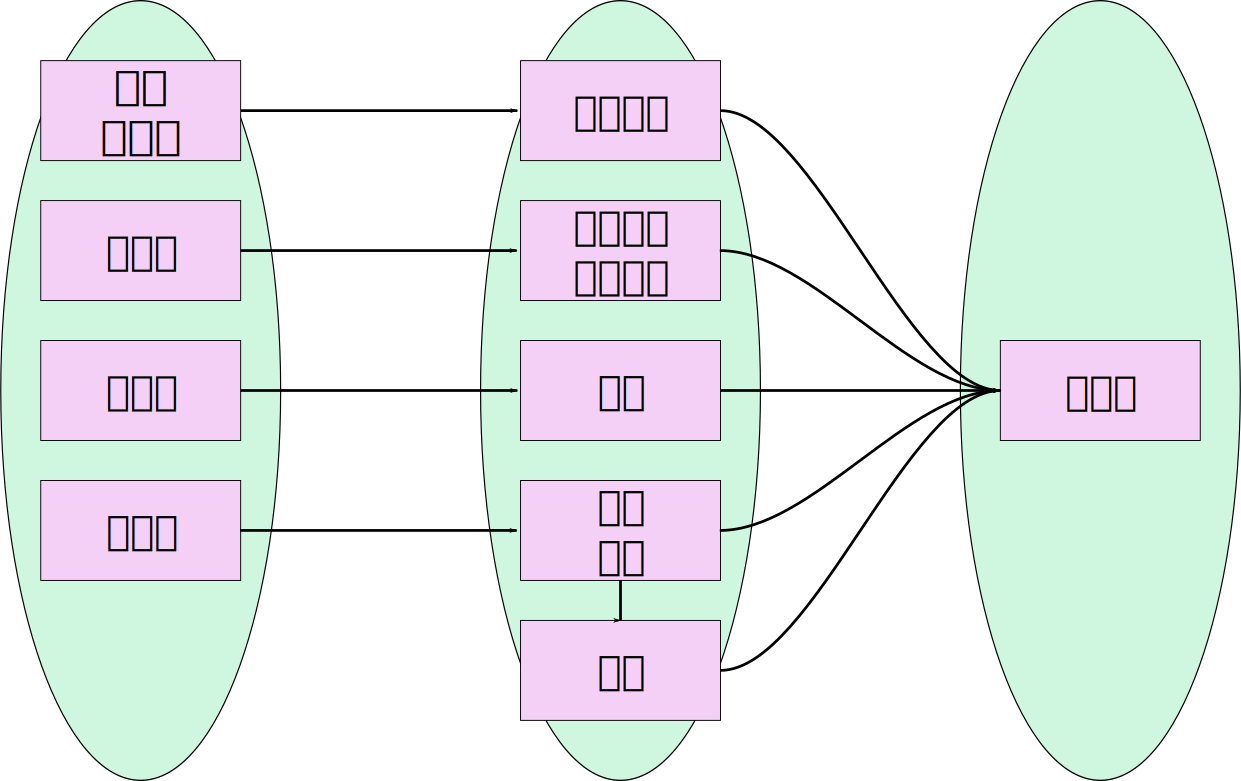
\includegraphics[keepaspectratio,width=40em]{圖/相關研究智識}}
\caption{逐門自然語言處理對應到相關的語言學}
\label{圖:相關研究智識}
\end{figure}

%漢語聲韻學→拼音系統
%語音學→語音合成、辨識
%音韻學→變調
%句法學→斷詞、剖析、翻譯
%語料庫

華語到閩南語的翻譯是自然語言處理(Natural Language Processing)\footnote{人講的話攏是自然語言}的一部份,
佇處理自然語言的時陣就需要語言相關的智識,會當簡單整理做圖\ref{圖:相關研究智識},
無仝的自然語言研究方向,愛知影的語言學智識嘛無仝。
紲落來就介紹語言學佮自然語言處理的研究文獻佮母語的研究狀況:

\section{音標系統}
\label{節:音標系統}
音標系統有兩種,一種是研究語音用的記音系統,一種是予一般人拼寫用的拼音系統。

\subsection{記音系統}
\label{小節:記音系統}
研究一个語言,愛先了解伊的語音,
這時陣就需要一个標準化的記音符號。
這馬上時行的是國際語言學會(International Phonetic Association)制定的
國際音標(International Phonetic Alphabet,IPA)\cite{WIKI國際音標},
毋管記錄的語言有仝款無,只要語音的特徵仝款,就會用仝款的符號。

\subsection{拼音系統}
\label{小節:拼音系統}
記音的音標符號較濟,有的符號是較罕得看著,用起來無方便。
實際寫文章、編教材大部份會用另外的音標系統。
下跤照歷史年代簡單介紹閩南語主要三種拼音系統:

\subsubsection{臺灣閩南語羅馬字拼音}
臺灣閩南語羅馬字拼音是中華民國教育部佇2008年發佈的拼音方案,簡稱做臺羅。
伊的前身是教會羅馬字(白話字)\cite{WIKI教會羅馬字}
佮臺灣語言音標(Taiwan Language Phonetic Alphabet,TLPA)\cite{WIKI臺灣語言音標},
這馬猶原相容教會羅馬字。


\subsubsection{方音符號}
方音符號,又稱方言音符號\cite{華、台語注音符號溯源}
將華語的注音符號閣加一寡聲母、韻母佮聲調符號來標注閩南語。
是1946年朱兆祥教授設計,
佇1998年時,中華民國教育部嘛捌公告使用過。

\subsubsection{通用拼音}
余伯泉教授\ji{⿱毛灬}頭,想欲統一華語、閩南語、客語佮原住民語的拼音系統。
中華民國教育部佇2002年到2008年規定華語通用拼音當做譯音標準。

%\subsubsection{音標比較表}
%國際音標 臺羅 方音 通用 例字


\section{語音學}
\label{節:語音學}

\begin{table}
\caption{元音表}
\label{表:元音表}
\centering
\begin{tabular}{c|ccc}
\diaghead{\theadfont Diag ColumnmnHead II}{喙舌懸低}{喙舌前後}
%喙唇扁/圓 
& 頭前 & 中央 & 後壁\\
\hline
懸 & [i] & [ɨ] & [u]\\
中懸 & [e] &  & [o]\\
中 &  & [ə] & \\
中低 & [ɛ] &  & [ɔ]\\
低 & [a] &  & [ɑ]\\
\end{tabular}
\end{table}

%\begin{table}
%\caption{輔音表}
%\label{表:輔音表}
%\centering
%\begin{tabular}{c|ccc}
%\diaghead{\theadfont Diag ColumnmnHead II}{發音方式}{喙舌所在}
%& 喙唇 & 中央 & 後壁\\
%\hline
%清塞音 & [i] & [ɨ] & [u]\\
%濁塞音 & i & ɨ & u\\
%鼻音 & [e] &  & [o]\\
%邊音 &  & ə & \\
%擦音 & ɛ &  & ɔ\\
%\end{tabular}
%\end{table}

\begin{table}
\caption{音節分析}
\label{表:音節分析}
\centering
\begin{tabular}{cccccc}
字 & 聲母 & \multicolumn{3}{c}{韻母} & 聲調\\
 & & 介音 & 主要元音 & 韻尾 &\\
\tsoo{良}{⿳⿳⿳ㄌㄧㆲˊ}{liong5} & [l] & [j] & [o] & [ŋ] & 5\\
\tsoo{媠}{⿳⿳⿳ㄙㄨㄧˋ}{sui2} & [s] & [u] & [i] & & 2\\
\tsoo{遠}{⿳⿳ㄏㆭ˫}{hng7} & [h] & & [ŋ̩] & & 7\\
\tsoo{意}{⿳ㄧ˪}{i3} & & & [i] & & 3\\
\end{tabular}
\end{table}

語音學(Phonetics)主要討論喙舌的運動方式佮語音的物理性質。

前國際語言學會會長John Ohala捌講過:
「語音變化是連續的(Continuous),為著研究只好假設做離散特徵(Discrete)的音素(Phoneme)。」
可比講「\tsoo{狗}{⿳⿳ㄍㄠˋ}{kau2}」,
音標寫做[kau],
實際上[k]佮[a]、[a]佮[u]中央有誠濟過渡的音,
毋過過渡的音實在傷濟,
無法度一个一个寫出來,
只好用[k]、[a]佮[u]三个符號代表「\tsoo{狗}{⿳⿳ㄍㄠˋ}{kau2}」的音標。

語音會當用氣流有順無,
大略仔分做元音(Vowel)佮輔音(Consonant)。
表\ref{表:元音表}是幾仔个閩南語定用的元音,
會當看著[i]佮[u]攏是喙舌較懸發的音,
而且喙舌佇i發音時比u發音閣較頭前,
這嘛影響著\ji{⿰因}的頻譜(Frequency Spectrum),
[i]佮[u]共振鋒(Formant)嘛小可無仝。
[i]佮[u]喙型嘛無仝,
唸「\tsoo{ㄨ}{}{u}」的時陣喙尖尖,
唸「\tsoo{ー}{}{i}」的時陣喙較平,
嘛影響著語音的變化。
%裂 sai sai:伊笑甲~~~
%裂喙:伊笑的時陣攏會~~

佇分析漢語的時,
會親像表\ref{表:音節分析}仝款,
共音節拆做聲母、韻母佮聲調來看,
韻母閣會當分做介音、主要元音佮韻尾。
毋過愛注意,
這个分析只是方便研究,
聲母、韻母的元素佮聲調猶原會互相影響。


若了解語音學,
就會當知影語音變化的道理,
支持音韻學的理論。

\section{音韻學}
\label{節:音韻學}

\begin{table}
\caption{閩南語上細配對}
\label{表:上細配對}
\centering
\begin{tabular}{c|cc}
& 喙唇 & 中央\\
\hline
元音、鼻化音 & [i](\tsoo{異}{⿳ㄧ˫}{i7}) & [ĩ](\tsoo{院}{⿳ㆪ˫}{inn7})\\
配合濁聲母 & [bi](\tsoo{味}{⿳⿳ㆠㄧ˫}{bi7}) & [mĩ](\tsoo{麵}{⿳⿳ㄇㄧ˫}{mi7})\\
\end{tabular}
\end{table}

現代的音韻學(Phonology)是對Ferdinand de Saussure\cite{de2011course}提出語言學研究,
必須分做共時(Synchronic Phonology)佮歷史(Diachronic Phonology)兩種音韻學。

\subsection{共時音韻學}
\label{小節:共時音韻學}
共時音韻學就是對一个時間的一个語言,
%討論變化,心中所想音檔→唸出來。
討論「頭殼底所想的音」到「唸出來的聲音」的語音變化。
佇討論語音進前,
咱就愛先訂出共時的語音單位,
定用的語音單位是音素。
音素代表一个人「頭殼底」,
對一个語言的「語音單位」。
愛判斷兩个音是毋是仝一个音素,
會當來揣「上細配對」。
可比講表\ref{表:上細配對}第一逝,
一般元音佮鼻化元音會當分出無仝的字,
所以[i]佮[ĩ]對人來講是辨識語音的單位,
是無仝的兩个音素。

\begin{equation}
\label{式:閩南語濁聲母變化式}
B\rightarrow\left\{\begin{matrix}
[b], & 佇一般元音頭前\\ 
[m], & 佇一般鼻化音頭前
\end{matrix}\right.
\end{equation}
\begin{table}
\centering
\caption{閩南語濁聲母無鼻化的選擇}
\label{表:閩南語濁聲母無鼻化的選擇}
\begin{tabular}{c|cc|c}
Bi+無鼻化 & 元音符合鼻音要求 & 規个音節鼻化一致 & 上好的選擇 \\
\hline
{[}bi{]} & & & ←是\tablefootnote{佇優選理論內底,←代表上好的選擇}\\
{[}bĩ{]} & *!毋是\tablefootnote{佇優選理論內底,*代表違反限制,!代表出局} & *毋是\cellcolor{gray}\tablefootnote{佇優選理論內底,殕色底代表選擇出局,毋免比} & \\
{[}mi{]} & & *!毋是 & \\
{[}mĩ{]} & *!毋是 & \cellcolor{gray} & \\
\end{tabular}
\caption{閩南語濁聲母有鼻化的選擇}
\label{表:閩南語濁聲母有鼻化的選擇}
\begin{tabular}{c|cc|c}
Bi+有鼻化 & 元音符合鼻音要求 & 規个音節鼻化一致 & 上好的選擇 \\
\hline
{[}bi{]} & *毋是 & \cellcolor{gray} & \\
{[}bĩ{]} & & *毋是 & \\
{[}mi{]} & *毋是 & *毋是\cellcolor{gray} & \\
{[}mĩ{]} & & & ←是\\
\end{tabular}
\end{table}

毋過看第二逝,
濁輔音佇[i]頭前是塞音[b],
佇[ĩ]頭前是變化鼻音[m],
因為無對比通證明[b]佮[m]有分辨字的能力,
所以[b]佮[m]對人來講「可能」是仝一个語音單位,
會當歸類做一个音素$B$\footnote{這个符號用m、b攏會使,伊只是代表一个音素},
只是$B$佇無仝的所在會唸無仝的音。

音韻學家就想欲揣出「頭殼底所想的音」到「唸出來的聲音」的關係,
討論為啥物面頂的$B$有時唸[b],有時陣唸[m],
目前較大的有衍生音韻學(Generative Phonology)佮優選理論(Optimality Theory)兩大派。

\subsubsection{衍生音韻學}
衍生音韻學是希望揣出的對應音韻規則(Phonological Rule),
親像面頂[b]佮[m]的問題會當看閩南語濁聲母變化規則\ref{式:閩南語濁聲母變化式},
$B$若後壁是一般元音,就變做[b],
若後壁是鼻化音,就變做[m]。

\subsubsection{優選理論}
第二派優選理論是揣出一寡人類語言通用的現象,
而且共這現象,
照重要程度排先後,
去揀人為啥物愛唸這个音。

可比講[b]佮[m]的問題,
咱有「元音符合鼻音要求」佮「規个音節鼻化一致」\cite{yip1996lexicon}兩个現象,
第一个現象「元音符合鼻音要求」是希望主要元音愛符合頭殼內有鼻音無鼻音的條件,
第二个現象「規个音節鼻化一致」是希望音節全部的音素,
\ji{⿰因}鼻化狀況是仝款的,
而且第一个現象比第二个現象優先,
若第一个現象無過,就免比第二个現象。

親像表\ref{表:閩南語濁聲母無鼻化的選擇},
假設頭殼底想的是「Bi+無鼻化」,
咱先產生[bi]、[bĩ]、[mi]、[mĩ]四个選擇\footnote{選擇其實閣有pi、pĩ、…無限濟个,\ji{⿰因}會用別的現象揀掉。為著簡單說明就無寫出來。},
其中[bĩ]佮[mĩ]違反第一个現象,
[bĩ]佮[mĩ]予人揀掉,
[bĩ]、[mi]違反第二个現象,
毋過因為[bĩ]早就違反第一个現象,
無需要閣判斷第二个現象,
所以第二个現象揀掉[mi]
上尾賰[bi],就是上好的選擇。
表\ref{表:閩南語濁聲母有鼻化的選擇}是「Bi+有鼻化」的例,
伊佇第一个現象揀掉[bi]、[mi],
第二个現象揀掉[bĩ],
上尾賰[mĩ]是上好的選擇。

\subsection{歷史音韻學}
\label{小節:歷史音韻學}
\begin{table}
\caption{閩南語低元音提昇過程\cite{hsieh2012low}}
\label{表:閩南語低元音提昇過程}
\centering
\begin{tabular}{ccc}
階段  & 音值 & 來源 \\
Stage 1 & jan/jat\tablefootnote{[i]的介音寫做[j]} &  Doty (1853), dictionary of Amoy dialect\\
Stage 2 & jan/jat &  Luo \& Zhou’s fieldwork in 1930 (L\&Z 1975)\\
Stage 3 & jen/jet & Taiwanese and some Southern Min dialects\\
Stage 4 & en/et & New forms among young Taiwanese speakers\\
\end{tabular}
\end{table}
\begin{equation}
\label{式:閩南語咸攝三等變化式}
[jaC]\rightarrow[jeC]\rightarrow[eC],若C\in\left\lbrace n,t\right\rbrace 
\end{equation}
\begin{equation}
\label{式:閩南語非咸攝三等變化式}
[jaC]\nrightarrow[jeC],若C\not\in\left\lbrace n,t\right\rbrace
\end{equation}
%[ja]\nrightarrow[je]

歷史音韻學是討論語言長期的變化佮語言互相的影響,
這个變化無一定是講話的人講無清楚,
嘛有可能是因為音相倚,
聽話的人聽毋著,
一緣一緣的人沓沓仔改變的。

親像表\ref{表:閩南語低元音提昇過程}記錄
閩南語「\tsoo{先}{⿳⿳ㄒㄧㄢ}{sian1}」佮「\tsoo{節}{⿳⿳⿳ㄐㄧㄚㆵ}{tsiat4}」韻母
這兩百冬的變化,
所以咱會當共這變化整理做規則\ref{式:閩南語咸攝三等變化式}。
除了寫出規則以外,
閣愛需要用語音學解釋為啥物會按呢生,
是因為頭前有介音[j],
喙舌佇較懸較頭前的所在\footnote{元音的所在會當看表\ref{表:元音表}},
後壁[n]佮[t]是舌尖音,
喙舌嘛是佇較懸較頭前的所在\footnote{舌尖音佮[i]、[j]的位較倚,讀者會當唸看覓[in]、[en]佮[an],觀察喙舌的變化},
予原本喙舌較低的[a],
變做喙舌較懸較頭前一寡的[e]。

毋過觀察別的韻煞無這種變化,
親像規則\ref{式:閩南語非咸攝三等變化式},
「\tsoo{閃}{⿳⿳⿳ㄒㄧㆰˋ}{siam2}」、「\tsoo{雙}{⿳⿳ㄒㄧㄤ}{siang1}」猶原是[jam]佮[jaŋ]。
用語音學的角度來看,
干焦頭前介音[j],無後壁的韻尾配合,
無法度予[a]變懸變做[e]。


\section{漢語聲韻學}
\label{節:漢語聲韻學}
聲韻學是研究漢語的歷史語言學,
參考韻冊佮現代漢語方言,
討論方言自古到現代的語音變化佮互相影響。

\subsection{韻冊}
\label{小節:韻冊}

聲韻學的主要研究材料就是韻冊,
韻冊會提供逐个字的聲母、韻母佮聲調資訊,
這就是聲韻學家會當提來推測古早漢語的發音系統的原因。

中國自三國南北朝時就有地區方言的韻冊\footnote{李登《聲類》、呂靜《韻集》},
到宋國官方綜合中國北方佮南方的語音系統的廣韻\cite{2002廣韻注漳州漢音}\cite{2010新校互註宋本廣韻},
廣韻是綜合各地的系統,
伊的聲母、韻母、聲調紀錄佇無仝的漢語方言攏會當用。

\subsection{古早中國語音紀錄}
\label{小節:古早中國語音紀錄}

\subsubsection{反切}
\label{小節:反切}

反切是古代中國用的記音方式,
記錄佇韻冊內底。
反切記音需要記兩个字,
一字代表聲母,一字代表韻母佮聲調,
親像閩南語的「\tsoo{東}{⿳ㄉㄤ}{tang}」會用「\tsoo{端}{⿳ㄉ}{t}」「\tsoo{通}{⿳ㄤ}{ang}」表示。%用「車」?

綜合各地的韻冊,
\ji{⿰因}記錄的反切嘛會當佇無仝的漢語方言用,
除了閩南語的「東」會當切做「端通」
華語的「\tsoo{東}{⿳⿳ㄉㄨㄥ}{}」嘛會當反切做「\tsoo{端}{⿳ㄉ}{}」「\tsoo{通}{⿳ㄨㄥ}{}」。

%\subsubsection{韻}
%\label{小節:韻}

%師詩斯


%狗頭後

%\subsubsection{攝等}
%\label{小節:攝等}


%\subsection{古早漢語推測}
%\label{小節:古早漢語推測}

%嘛因為韻冊的紀錄攏毋是實際發音音值,
%誠濟聲韻學家以語音學佮音韻學的理論,
%參考韻冊佮現代方言,
%來推測古早漢語的發音系統。
%
%ian ien en

%\section{句法學}
%\label{節:句法學}
%句法學就是討論啥物是詞、詞的用法、句型的結構。
%親像
%
%陸儉明


\section{機器學習}
\label{節:機器學習}
自然語言的問題定定非常複雜,
有的時陣無法度揣著規則來解決。
這个時陣就會當共資料交予電腦來判斷。

這節就簡單介紹分類器佮隱性馬可夫模型:

\subsection{分類器}
\label{小節:分類器}
分類器是機器學習的一類研究,
先決定分類器的模型生啥款,
模型內底有誠濟參數,
予伊訓練資料,
訓練資料內底有一堆問題佮對應的答案,
分類器會用輸入訓練資料的問題,
揣出上適合的參數, 
予輸入的問題會當用這參數對應到訓練資料的答案。
等待後壁有新的問題入來時,
分類器會用伊訓練出來的參數來算答案。

定用的分類器模型有
高斯混合模型(Gaussian mixture model,GMM)、
決策樹(Decision Tree,DT)、
支持向量機(Support Vector Machine,SVM)佮
深層學習(Deep learning),
逐个分類器的專長無仝,
應用的所在嘛無仝,
會當看表\ref{表:定用的分類器優缺點}。

\begin{table}
\caption{定用的分類器優缺點}
\label{表:定用的分類器優缺點}
\centering
\begin{tabular}{ccc}
分類器 & 優點 & 缺點 \\
高斯混合模型 & 知影「結果正確」的機率 & 訓練的過程無一定收斂 \\
決策樹 & 輸入會當是字串、符號 & 訓練資料的答案數量愛平均分配\\
支持向量機 & 效果好,效果閣穩定 & 答案的種類無法度傷濟\\
深層學習 & 效果上好 & 訓練資料愛非常濟,使用門檻非常懸\\
\end{tabular}
\end{table}
%\subsubsection{支持向量機}
%\label{小節:支持向量機}
%
%\subsubsection{決策樹}
%\label{小節:決策樹}
%
%\subsubsection{高斯混合模型}
%\label{小節:高斯混合模型}

\subsection{隱性馬可夫模型}
\label{小節:隱性馬可夫模型}
隱性馬可夫模型(Hidden Markov Model,HMM)是針對有狀態轉移的問題,
毋過咱看袂著「狀態」本身,
咱只會當看著佮狀態有關係的「現象」。
隱性馬可夫模型就是想欲用咱看著的現象,
去推測實際的狀態倒底是按怎變化。

%\cite{HMM}
%例


\section{語音辨識}
\label{節:語音辨識}
語音辨識(Speech Recognition)就是共語音轉做文字,
會當用佇語音指令佮問答系統\footnote{親像蘋果公司的Siri}。

語音辨識主要的做法是揣出語音佮音標的對應,
共語音轉做一个一个MFCC聲學特徵,
%\footnote{用MFCC特徵\cite{MFCC特徵}是因為實驗的效果上好\cite{MFCC上好}}
用分類器去判斷是佇一个音標。

因為語音訊號連續閣無固定長度,
為著解決這个問題,
就假設語音變化是狀態的轉移,
用隱性馬可夫模型來模擬語音狀態的變化。

這方面的開源工具有HTK佮Kaldi:

\subsection{HTK}
\label{小節:HTK}
HTK全名號做Hidden Markov Model Toolkit\cite{young2006htk},
發展的時間較早\footnote{對1989年到最近上新的2009年版本},
伊主要用的高斯混合模型當做分類器,
而且用決策樹合併相倚的高斯模型。

%HTK的模型訓練腳本\footnote{會當參考附錄\ref{章:臺灣言語工具}的臺灣言語工具,內底有提共HTK訓練佮使用的腳本},
%一開始會先照文本的音,共音檔平均切做一个一个,
%HTK流程圖~~

%決策樹
%wfst

\subsection{Kaldi}
\label{小節:Kaldi}
Kaldi\cite{Kaldi:Povey_ASRU2011}是較新的工具,
除了訓練一開始嘛是佮HTK仝款用高斯混合模型以外,
伊訓練後壁閣加入深層學習佮其他的演算法,
效果比HTK閣較好。


%SGMM

\section{語音合成}
\label{節:語音合成}
語音合成(Speech Synthesis)是佮文字轉做聲音,佮語音辨識顛倒反。
親像車站廣播,有聲冊攏是語音合成的應用。
這馬時行的做法有模型合成(Model-based Speech Synthesis)佮接音合成(Corpus-based Speech Synthesis)兩種:

\subsection{模型合成}
\label{小節:模型合成}
這个方法揣出音標\footnote{用人工抑是語音辨識軟體標記}佮語音的對應關係,
啥物音標會唸啥物音。
頭一步是用合成器(Vocoder)共語音訊號轉做一个一个的頻譜佮頻率,
才用隱性馬可夫模型佮分類器,
共音標當做輸入,
頻譜佮頻率當作輸出訓練隱性馬可夫模型佮分類器的參數。
等欲合聲音時,才閣照模型的特徵,
用合成器合聲音出來。

伊的輸出語音,
韻律攏誠自然,
毋過聲音的品質比原本語料的音質較\ji{⿰禾黑}一寡,
因為訓練的時,
聲音先用合成器轉做特徵,
合成的時,
特徵閣用合成器轉語音,
兩擺轉換造成音質變\ji{⿰禾黑}。

\subsubsection{HTS}
\label{小節:HTS}
這方面開源軟體有HTS(HMM-based Speech Synthesis System)\cite{hts_zen2007hmm},
伊是對HTK修改來的,
仝款用隱性馬可夫模型、高斯混合模型佮決策樹。
%合成器用SPTK
%用mgc、lf0、duration做聲音特徵,
%
%伊訓練方式,
%伊一个聲音會分做5个state\footnote{下跤講著的5狀態、三連音,攏是參數,毋是固定的},
%逐个state有一个高斯模型,
%伊會先訓練逐个音的初步模型,
%閣來訓練三連音模型,
%閣用決策樹共相倚的音綁做伙。
%
%合的時陣才閣查決策樹,
%共mgc、lf0、duration查出來,
%閣用合成器合語音出來。
%莫用GV

HTS有3000~7000句的訓練語料,
就會當得著袂\ji{⿰禾黑}的效果,
缺點若有聲音效果\ji{⿰禾黑},歹除錯。

%伊需要音檔,標記發音內容的音檔,閣有音類的問題集。設計標仔。
%標仔的時間會使對HTK訓練。
%根據經驗,3000句會使,5000句普通,7000句上好。

\subsection{接音合成}
\label{小節:接音合成}
模型合成有音質的問題,
為著保持音質,
接音合成共原本的音檔庫切做一个一个細音檔,
合成的時陣,
提細音檔來接起來。

對漢語來講,
只需要共逐種音錄起來就好矣,
毋過一字一字聽起來無順無自然。

為著改善接起來韻律無自然的問題,
接音合成會配合模型合成,
用模型產生的韻律,
揀接起來較自然的細音檔。
按呢做的優點是聲音品質誠好,
缺點是語料愛有夠,
因為需要誠濟的細音檔來配合韻律,
若拄著合成品質無好的語句,
就錄音增加音檔庫就好矣。

\subsection{變調佮重音預測}
\label{小節:變調佮重音預測}
佇書寫的音標佮實際唸的發音定定是無仝款的,
上大的差別就是聲調佮重音。
親漢語有聲調,
聲調到發音之間有變調的問題。
南島語有重音,
標註語句的重音嘛是一个音韻學的研究問題。

用閩南語做例,
準做想欲共閩南語的音標變做閩南語的聲音,
毋過實際的音標到唸的發音閣無仝,
後且閩南語的變調傷過複雜的,
需要專門的處理。

楊允言教授就有做過閩南語的變調系統\cite{iunn:台語變調系統實作研究},
用斷詞、詞性佮句型的資訊,
配合20類音韻規則來變調,
得著88.90\%的結果。
音韻規則的優點是語料無蓋濟的時,
就會當得著八九成的正確率,
毋過若數量一濟,
規則的先後會較歹處理。

變調嘛會當用分類器來做,
共規則式用著的特徵當做參數下入去,
看佗一个分類模型會較好。
伊上大的好處就是管理方便,
拄著新語料,重訓練模型就好矣,
缺點是訓練資料需要誠濟。

\subsection{相關系統}
\label{小節:語音合成相關系統}
目前臺灣母語的語音合成只有閩南語佮客話,
親像表\ref{表:語音合成研究、系統},
頭前三个攏是用接音合成,配合字的錄音
第四第五个是接音合成配合韻律模型
上尾一个主要是訓練閩南語HTS模型。

因為南島語的語料較少,
嘛無法度親像漢語幾字仔錄音就有基本的效果,
就需要請專人來錄音、整理,
這是咱閣愛拍拼的所在!

\begin{table}
\caption{臺灣母語語音合成相關研究、系統}
\label{表:語音合成研究、系統}
\centering
\begin{tabular}{ccc}
1999 & 林川傑 & 閩南語翻譯佮語音合成系統\cite{中文到閩南語之線上翻譯及閩南語之語音合成} \\
2002 & 李雪貞 & 客家語語音合成之初步研究\cite{李雪貞2002客家語語音合成之初步研究} \\
2005 & 楊允言、劉杰岳佮李盛安 & 台語羅馬字發音試驗系統\cite{楊允言_台語羅馬字發音試驗系統} \\
2008 & 陳信宏、余秀敏佮羅烈師 & 客語文句轉語音及語音辨認之研究\cite{陳信宏2008客語文句轉語音及語音辨認之研究} \\
2010 & 蔡依玲 & 基於隱藏式馬可夫模型之客語文句轉語音系統\cite{蔡依玲2010基於隱藏式馬可夫模型之客語文句轉語音系統} \\
2013 & 薛丞宏 & 意傳文化科技\cite{意傳文化科技}
\end{tabular}
\end{table}

\section{斷詞}
\label{節:斷詞}
斷詞是共語句照一个詞一个詞分開的技術,
親像漢語佮日語的文字定定是一字一字無分開,
就看袂出來倒底佗一字佮佗一字是一个詞,
若愛提著詞的資訊,
就需要程式來斷詞。
斷詞的效果嘛會影響著翻譯、變調佮其他技術的效果。

有一寡語言現象是佮詞有關係,
親像閩南語的變調,
毋過漢語語句的文本,

所以就需要斷詞,
共詞佮詞分開,
後壁的應用才有法度繼續落去。



%轉格式
%斷詞前
%自稱一世人離袂開預報工作的吳德榮
%tsu7 tshing1 tsit8 si3 lang5 li5 be7 khui1 ...
%斷詞後
%自稱 一世人 離袂開 預報 工作 的 吳德榮
%tsu7-tshing1 tsit8-si3-lang5 li5-be7-khui1 ...


華語這方面有中研院中文斷詞系統(CKIP)\cite{CKIP論文}。

閩南語斷詞的標準,
自誠早以前就有人討論矣\cite{台語斷詞原則討論},
教育部嘛有出「臺灣閩南語羅馬字拼音方案連字符使用原則」\cite{臺羅拼音},
定義連字符的標準。

%斷詞的標準有誠濟種,為著方便,以教育部的「臺灣閩南語羅馬字拼音方案連字符使用原則」的連字符當做一个詞,若「tsiah8 png7」(食白米飯的意思),當做兩个詞,「tsiah8-png7」(食物件的意思),當做一个詞。


%斷詞方法:長詞優先、配合語言模型、統計式、馬可夫、詞性

\subsection{長詞優先斷詞}
\label{節:長詞優先斷詞}

定看著的斷詞方法有上長詞優先(Maximum Matching),
伊的做法是自後頭開始看\footnote{華語實驗的結果,自後頭開始的效果比對頭前的閣較好},
往頭前幾个字是毋是會當揣著一个佇辭典的詞,
若會使,就揀上長的彼个,
希望詞愈長愈好,會當看方法\ref{方法:長詞優先斷詞方法}。

%解釋比如說,『我想要吃飯』可以切成『我,想,要,吃,飯』『我,想要,吃飯』『我,想要吃飯』『我想要,吃飯』『我想要吃飯』,其中,能夠在字典找到詞的切割方式有『我,想,要,吃,飯』『我,想要,吃飯』,

\begin{algorithm}
  \caption{長詞優先斷詞方法}
  \label{方法:長詞優先斷詞方法}
  \begin{algorithmic}[1]
    \REQUIRE 無斷詞的語句$[j_{1}, j_{2}, ... , j_{m}]$
    \ENSURE 斷詞的語句$[s_{1}, s_{2}, ... , s_{n}]$
    \STATE \( 決定辭典上長的詞字數$k$ \)
    \STATE 揣一个上細的\(i\),予\(j_{i+1}, j_{i+2}, ... , j_{m}\)是辭典的一个詞,而且\(m − k ≤ i ≤ m − 1\)
    \STATE 斷詞的語句加入\(s=j_{i+1}, j_{i+2}, ... , j_{m}\)
    \STATE \( $m=i$ \),重做第1步,到\(i=0\)為止
  \end{algorithmic}
\end{algorithm}


%\section{詞性標記}
%\label{節:詞性標記}
%\subsection{相關系統}
%\label{小節:詞性標記相關系統}
%\cite{iunn:利用統計方法及中文訓練資料處理台語文詞性標記}
%

\section{剖析}
\label{節:剖析}
剖析是了解語句內底詞的關係,
分析語句的句型。
剖析會當用佇翻譯佮語意分析,
較定看著的就是問答系統\footnote{親像蘋果公司的Siri}。

做剖析需要句法學的知識,
閣愛有一致的人工檢查,
這是一个誠大的工程。

%http://nlp.stanford.edu/software/stanford-dependencies.shtml#Download
%http://stackoverflow.com/questions/10401076/difference-between-constituency-parser-and-dependency-parser
\subsection{相關系統}
\label{小節:剖析相關系統}
楊允言教授捌做過閩南語的剖析樹仔\cite{台語文語法結構樹建置},
毋過數量猶原無夠,需要閣整理。

一開始的語料歹收集,
有一个辦法是借用華語的剖析,
先共閩南語翻譯做華語,
才閣共華語語句的剖析樹仔\cite{chen2005chinese}對應去閩南語語句,
按呢就有初步的樹仔矣。
訂好剖析樹仔規則了後,
就會使整理初步的樹仔,
等待資料有夠濟,
就會提樹仔的語料來訓練一个閩南語的剖析器\cite{klein2003accurate}。

%人工若校對,全部的資料著愛收集起來
%而且嘛愛親像XX節的XX圖仝款,愛做一个改錯誤的程式,予人工莫一直改仝款的物件
。

\section{翻譯}
\label{節:翻譯}
這馬電腦時行的翻譯方式是統計式機器翻譯(Statistical Machine Translation),
這是對1993年Brown用數學證明\cite{brown1993mathematics}開始,
一直發展到這馬。
統計式機器翻譯會當分做對齊模型(Alignment Model)、語言模型(Language Model)佮解碼器(Decoder)三个部份:

\subsection{對齊模型}
\label{小節:對齊模型}
對齊模型的功能是予解碼器知影詞愛按怎翻譯,
可比講是一个雙語的辭典。

對齊模型有分斷詞對齊佮剖析樹對齊兩種,下跤用斷詞對齊說明伊的原理。

先準備一組一組的華語閩南語平行語料,
親像「我 要 吃飯」和「我 欲 食 飯」,
紲落來產生語詞對照表。
華語詞的「要」,會對應到「我」、「欲」、「食」、「飯」閩南語詞,
經過大量的平行語料,
上尾知影華語的「要」定定對應著閩南語的「欲」,
也就是共對應頻率懸的組合留落來。
%改例

開源工具GIZA++\cite{och2003systematic}實作Brown 1993的演算法,
而且這馬嘛有支援多核心的MGIZA\cite{gao2008parallel}。

\subsection{語言模型}
\label{小節:語言模型}
第二部份是語言模型(language model),伊是欲用來判斷一句話是好是\ji{⿰禾黑}。

%加數學解釋
伊的做法是去記錄逐个詞後壁定定會接啥物詞,
若有一句話是「…欲 食…」,有「欲」佮「食」兩个詞,
咱知影「…欲 食」的後壁接「飯」比「…欲 食」的後壁接「湯」的機率較大,
也就是講「欲 食 飯」連紲詞比「欲 食 湯」連紲詞機率大,
若語言模型一擺看「欲 食 飯」三个詞,
就是三連紲詞模型(3-grams model)。
語言模型判斷一句話,伊出現的機率有偌大,就是看這句話伊內底連紲詞的機率是偌大。
%改例

這方面的工具有IRSTLM\cite{federico2008irstlm}、
SRILM\cite{stolcke2002srilm}佮
KenLM\cite{Heafield-estimate},
其中IRSTLM佮KenLM是LGPL開放授權,
SRILM是學術授權。

\subsection{解碼器}
\label{小節:解碼器}
上尾一部份是解碼器,
提面頂講的對齊模型、語言模型,
來翻譯華語到閩南語。

因為翻譯的問題毋是多項式時間(NP problem)會當解出來的,
所以解碼器袂使硬算全部的可能,
必須用有效率的演算法來翻譯。

上有名的開源程式就是Moses\cite{Koehn:2007:MOS:1557769.1557821},
伊整合對齊模型佮語言模型的介面,
閣有專工的訓練包通使用\cite{Moses訓練包}。

\subsection{評分方式}
\label{小節:評分方式}

翻譯大部份攏用BLEU(Bilingual Evaluation Understudy)來評分,
伊用連紲詞的概念來評分,
$BLEU=100\times{e^{\max{0,\frac{\textit{結果-答案長度}}{\textit{結果長度}}}}}\times{\sum_{n=1}^{4}(\textrm{n連紲詞})^{\frac{1}{4}}}$\cite{BLEU程式}。
%改cite

準若翻譯的答案是「這 幾 工 寒流 閣再 展威」,咱有兩个翻譯的結果,翻譯結果一「這 幾 工 寒流 有 展威」佮結果二「寒流 這 幾 工 閣再 展威」,請看表\ref{表:範例BLEU分數},答案有「這 幾 工」、「幾 工 寒流」、「工 寒流 閣再」佮「寒流 閣再 展威」4个三連紲詞,結果一有出現2个,所以結果一的三連紲詞分數是2/4,結果二有出現1个,分數是1/4。因為結果二無對應的四連紲詞,伊的分數都比結果一低。

\begin{table}
\caption{翻譯結果一「這 幾 工 寒流 有 展威」佮翻譯結果二「寒流 這 幾 工 閣再 展威」對答案「這 幾 工 寒流 閣再 展威」的分數}%
\label{表:範例BLEU分數}
\centering
\begin{tabular}{|c|cccc|c|}
\hline
翻著的數量 & 一連紲詞 & 兩連紲詞 & 三連紲詞 & 四連紲詞 & BLEU分數\\
\hline
結果一 & 5/6 & 3/5 & 2/4 & 1/3 & 53.73\\
\hline
結果二 & 6/6 & 3/5 & 1/4 & 0/4 & 0.00\\
\hline
\end{tabular}
\end{table}

\section{語料收集整理}
\label{節:語料收集整理}
%佇這个網路的時代,收集語料上緊的方法就是去網路面頂掠。看圖XX,先共閩南語專門的字詞擲去搜尋引擊\footnote{親像Google、Bing},閣照揣著的網頁去掠相關的閩南語。
%閩南語的網頁內底除了閩南語以外,有可能閣濫一部份的華語,為著莫予華語語料影響著閩南語模型,所以愛想辦法共臺華兩種語言分開。分開了後
%
%%圖:關鍵詞 引擊 網址 掠網頁 網頁html 轉文字 一句一句的語料 判斷語言 閩南語/華語 對齊
%
%\begin{figure}
%\centerline{\includegraphics[keepaspectratio,width=40em]{圖/網路語料庫結構}}
%\caption{網路語料庫}
%\label{圖:網路語料庫結構}
%\end{figure}
%
%\subsection{收集網路資料}
%\label{小節:收集網路資料}

\subsection{語言分類}
\label{小節:語言分類}
語言分類(Language Identification)是輸入一句話,
判斷是佗一種語言。
這馬上時行的方法是以字元為單位,語言模型算分數\cite{cavnar1994n}

南島語主要嘛是拼音文字,
所以會使用這个方法,
南島語佮漢語的語言分類較簡單,
就算漢語用羅馬拼音,
拼音的種類嘛差誠濟,
只要檢驗有聲調抑是拼音規則就會使判斷是南島語抑是漢語。

\subsection{平行語料語句對齊}
\label{小節:語句對齊}
翻譯語料的平行語料需要一句一句對齊,
若原本的語料是一篇一篇對應的,
就需要平行語料語句對齊(Parallel Corpus Sentences Alignment)。

語句對齊的方法有誠濟種,
有照字元數量對齊的Gale and Church算法\cite{gale1993program},
嘛有用翻譯結果輔助的Bleualign\cite{zora38464}。

\section{語料庫}
\label{節:語料庫}
自然語言處理需要語料才有法度訓練模型,
就需要語料庫共語料存起來。

\begin{table}
\caption{自然語言處理技術需要的語料庫}
\label{表:自然語言處理技術需要的語料庫}
\centering
\begin{tabular}{lc}
技術 & 語料樣式 \\
變調 & 原始文本、本調音標佮變調音標 \\
語音辨識 & 濟人音檔佮對應文本 \\
語音合成 & 孤人音檔佮對應文本 \\
斷詞 & 斷詞的語料 \\
剖析 & 剖析樹 \\
翻譯 & 兩種語言的平行語料 \\
\end{tabular}
\end{table}

有的語料庫是純文字的資料庫,
嘛有存音檔的語料庫,
愛看需求,定看著的技術會當參考表\ref{表:自然語言處理技術需要的語料庫}。

\subsection{閩南語語料種類}
\label{節:閩南語語料種類}

\begin{table}
\caption{閩南語語料種類比較表}
\label{表:閩南語語料種類比較表}
\centering
\begin{tabular}{lcc}
種類 & 範例 & 備註\\
全漢 & 我欲食飯 & 全部漢字\\
全羅 & gua2 beh4 tsiah8-png7 & 全部羅馬拼音,有斷詞資訊\\
漢羅 &我beh4食飯 & 漢字拼音濫咧用\\
\end{tabular}
\end{table}

閩南語是漢語的一支方言,
大部份的字攏會當揣著漢字,
毋過閩南語嘛毋是純漢語,
有的字無對應的漢字。

有的人慣勢全部用羅馬拼音創作,
這種寫法號做「全羅」。
嘛有人慣勢全部用漢字創作,
號做「全漢」
毋過有的字無法度揣著對應的漢字,
全漢實際上的拄著造字、揣字的困難,
為著創作方便,
知影的字用漢字寫,
賰的用音標寫落來,
號做「漢羅」。
詳細會當看表\ref{表:閩南語語料種類比較表}的範例。

\subsection{閩南語語料-新聞語料庫}
\label{節:新聞語料庫}
iCorpus臺華平行新聞語料庫(後壁用「新聞語料庫」稱呼)\cite{iCorpus臺華平行新聞語料庫}
是中央研究院資訊所陳孟彰老師主持,內底的文章主要是何澤政翻譯的。

何澤政\footnote{一九七零年代出世,臺中烏日人}對民國九十七年十一月初六開始,
逐工揣兩篇華語新聞,先人工斷詞斷句,
後尾翻譯做閩南語教會全羅,
罕得改變用詞的先後。

親像原本的新聞「這幾天寒流再度發威」,翻譯做「tsit4-kui2-kang han5-liu5 koh-tsai3 tian2-ui」(這幾工寒流閣再展威)\footnote{原文是教會羅馬字,為著文章一致,以教育部的臺羅書寫}。
%新聞語料庫的翻譯,親像面頂的「這幾天寒流再度發威」,較袂翻做「寒流這幾工閣再展威」,除非照華語用詞先後翻譯的結果無順,才會調整。

澤政佇語料內底用
「挕捒 hinn3-sak4」%轉格式
\footnote{挕捒意思共物件擲掉、放捒,嘛就是華話的「丟棄」
%,例句甲(家己做的):這支筆好好,為啥物愛共伊挕捒。
%例句乙(Tek-hôa,Nah ē teh批判民進黨?,\url{http://taioan-chouhap.myweb.hinet.net/089.htm}):民進黨接續李登輝的路線, 繼續加強黨國時代權力者, 倚附者佮既得利益者的優勢,毋是共刜挕捒。
}
、
「作孽tsok4-giat8」%轉格式
\footnote{
%青-少-年|tshing1-siau3-lian5 作-孽|tsok4-giat8 跤-踏-車|kha1-tah8-tshia1 擲|tan3 落|loh8 河-中|ho5-tiong1。
%拄著外來詞,澤政嘛會選擇保留原文,拄著華語的「歐巴馬」佮「西藏」,會翻轉去英文「Obama」、「Tibet」。
%愛耍手賤,華語的「惡作劇」。例句甲:叫你莫摸你閣摸,誠實手賤愛作孽!(家己做的)例句乙:你這个作孽囡仔,你是按怎沐甲一身軀烏趖趖?(惠光,天真瀾漫,\url{http://ip194097.ntcu.edu.tw/nmtl/DADWT/thak.asp?id=992})
}
本土的詞以外,伊嘛會配合這馬發生的代誌,用較時行的閩南語,親像
「喙罨」\footnote{華語的「口罩」}、%轉格式
「心肌梗窒心|sim1 肌|ki1 梗|king2 窒|that4」\footnote{華語的「心肌梗塞」}、%轉格式
「自來水」\footnote{閩南語較古典的用法,會號做「水道水」}、…。%轉格式

而且除了現代閩南語,澤政伊閣會去查台華線頂辭典\cite{台華線頂辭典}
選擇較古典的用詞\footnote{台華線頂辭典是古早語料,一个詞若台華線頂辭典查有,教育部辭典查無,就當做伊是較古典的詞},親像
「𤺪|sian7 篤-篤|tauh4-tauh4」%轉格式
%\footnote{熱-天|juah8-thinn1 高-溫|ko1-un1 炎-熱|iam7-juah8 規-工|kui1-kang1 𤺪|sian7 篤-篤|tauh4-tauh4 。|。}
、
「鬥-贊-手|tau3-tsan3-tshiu2」。%轉格式
%\footnote{佇|ti7 三|sam1 一-一|it4-it4 大-地-動|tua7-te7-tang7 慷-慨|khong2-khai3 鬥-贊-手|tau3-tsan3-tshiu2 ,|,}。
拄著外來詞,澤政嘛會選擇保留原文,
拄著華語的「歐巴馬」佮「西藏」,
會翻轉去英文「Obama」、「Tibet」。

%若源頭是日本話外來詞,就會直接用教羅寫出來,請看

\subsection{閩南語語料-教育部辭典}
\label{節:教育部辭典}
教育部辭典全名「臺灣閩南語常用詞辭典」\cite{教育部臺灣閩南語常用詞辭典},
正式版是100年上線,
伊有25892的詞條\footnote{1021230的資料},
內底誠濟生活的用語,
大部份詞條攏有漢字、音標、解釋、例句佮翻譯。

這个辭典是教育部編的,當然漢字有照教育部家己的規範\footnote{臺灣閩南語推薦用字700字表,佇96~99年公佈修正}來寫,所以伊內部的用字前後有一致,為著翻譯的效果佮使用者的方便,就共教育部辭典的用字當做標準,若有用字佮教育部的用字無仝的,就改做教育部的用字。%//閣愛順過

伊的例句,除了閩南語漢字佮音標以外,閣有敆華語的翻譯,親像表\ref{表:教育部辭典例句},漢字佮音標的對應會使提去做用字參考的字典,音標的部份會當提來斷詞,訓練語言模型,閩南語佮華語的對應會使提來做平行語料。
嘛因為伊有漢字佮音標,就會當共遮的漢字佮音標收集起來,當做用字參考的字典,
\begin{table}
\caption{教育部辭典例句}
\label{表:教育部辭典例句}
\centering
\begin{tabular}{l}
彼个查某囡仔真媠。 \\
Hit ê tsa-bóo gín-á tsin suí.\\%轉格式
那個女孩子很漂亮。\\
\end{tabular}
\end{table}

除了一般的詞條以外,教育部辭典嘛有收一寡俗語、臆謎猜,攏做388句做附錄句。
因為附錄句干焦提供解釋,所以無法度提來做平行語料,毋過會使提來訓練語言模型。


\subsection{閩南語語料-臺文典藏}
\label{節:數位典藏}
台語文數位典藏資料庫(下跤號做臺文典藏)\cite{台語文數位典藏資料庫}
是國家臺灣文學館收集1885~2006年的語料。
臺文典藏的來源語料百百款,攏總2167篇,
照時代分做清國時期170篇、日治時代490篇,民國統治1507篇。
內底嘛有照語料形式分做四類,有詩387條、散文1127篇、小說387篇、劇本49篇。%攏總416343句。

因為伊是百外冬的語料庫,較古早的語料,用詞就較古典,
格式嘛無仝,有的是漢羅,有的是全羅。
臺文館\ji{⿰因}因為著格式統一,
就替原底是全漢抑是漢羅的語料補全羅拼音\footnote{有時陣劇本邊仔的解釋會用漢字,親像「(福哥仔出場)」}。
若原本是全羅,就請人拍漢羅,會當看表\ref{表:數位典藏語料},
拍漢羅的時,\ji{⿰因}若知影漢字,就會拍漢字,
賰的外來語,抑是較本土的語詞就會用音標來拍。
伊有的語料是一句對齊一句,有的是一段對齊一段。

\begin{table}
\caption{數位典藏語料漢羅、全羅對照}
\label{表:數位典藏語料}
\centering
\begin{tabular}{l}
漢羅:Koh m7知u7危險.........., \\
全羅\footnote{臺文典藏內底原本是教會羅馬拼音,為著讀者方便,攏改做教育部的臺羅}:Koh m7-tsai u7 gui5-hiam2...............,\\
\end{tabular}
\end{table}


\subsection{閩南語語料-TGB通訊臺灣組合}
\label{節:TGB通訊-臺灣組合}
TGB通訊\cite{TGB通訊}是學生台灣語文促進會
對1999年10月開始\cite{學生台灣語文促進會對1999年10月開始}\footnote{\url{}}
一個月一期的刊物。
頭前60期以閩南語為主,61期後有提供華語對照,
有時陣閩南語句內底會濫一寡華語詞,形式較無固定。


%因為有閩南語、有華語佮臺華平行語料,嘛閣有濫做伙的, 誠濟種實際會拄著的情形會當提來做判斷語言的語料。
%有的時陣閩南語佮華語濫做伙,先定義啥物情形算閩南語,啥物情形算華語

%用人工分
%
%主要語句是閩南語,有一兩个詞是華語嘛是算閩南語
%閩南語
%
%聽人講 khah 早有出現過『小蜜蜂』
%我 beh tńg 來種作 ! ── 記 0312 Truku 反亞泥 ‧ 還我土地運動
%有台灣味 ê 繪本──《我和我的腳踏車》 .
%
%華語
%華語閩南語攏通的算華語
%有華語完整的一句話就算華語
%毋是華語嘛毋是閩南語,親像英文、日語、…
%
%「 糟了 ,是工地火燒厝, 緊轉去打 火 ! 」建設公司 的 工地主任 從手機接到消息,通話結束後就帶著那群混混先離開了。
%『聽說妳最近遇到什麼問題 , 是不是 ? 怎麼了 ? 』好性地 ê QA 繼續問--落-去 .
%去越南胡志明市 4 工/越南胡志明市四日行 @Gio̍k-hōng

%\subsection{閩南語語料腔口統計佮處理}
%\label{小節:閩南語語料腔口統計佮處理}






\chapter{研究介紹}
\label{章:研究介紹}

咱的目標是予閩南語的翻譯,效果閣較好,
效果的好\ji{⿰禾黑}是看BLEU拍的分數\footnote{請看\ref{小節:評分方式}節的紹介}。

佇遮希望預處理語料,
予翻譯效果變好。
統計式機器翻譯的效果決定佇統計的模型,
若愛翻譯翻較好,有兩个大方向通做:
第一个方向是予語料的形式相像,
若語料的形式愈仝款,
翻譯的統計機率會閣較好。
第二个方向是資料愈濟愈好,
加新的語料庫了後,
翻譯模型有法度揀著上好的語詞來翻譯。

本章第\ref{節:閩南語斷詞}摻\ref{節:未知詞問題}節針對第一个方向做,
因為閩南語目前閣無剖析的程式,
本論文對齊模型用的是斷詞翻譯\footnote{請看\ref{節:翻譯}節的紹介},
語料的樣式就是以斷詞為主。
\ref{節:閩南語斷詞}節討論一種斷詞方法,
對閩南語數量無濟的語料上好的問題。
\ref{節:未知詞問題}節說明斷詞的語料翻譯,
一寡詞會翻袂出來的問題。
第二个方向是第\ref{節:整理語料}和\ref{節:分類語言}節,
\ref{節:整理語料}節講摻別的語料庫時,
會發生啥物問題。
\ref{節:分類語言}節對網路頂掠落來的資料,
愛按怎共語料照語言分類。


\section{閩南語斷詞}
\label{節:閩南語斷詞}
咱若共\ref{節:改變語料格式}節佮\ref{節:未知詞另外翻譯}節的方法合做伙,效果上好的是斷詞組對斷詞組,毋過斷詞組需要用剖析器去揣結構樹,閣來定規則決定詞佮詞啥物時陣愛敆做伙變詞組,這就是另外一門學問矣。目前閩南語閣無這資源,自然賰「華語斷詞-閩南語斷字」佮「華語斷詞-閩南語斷詞」上好,準若有好的斷詞工具,閩南語斷詞模型應該愛比閩南語斷字模型閣較好,雖然佇這擺實驗斷詞模型顛倒較\ji{⿰禾黑},毋過為著未來閩南語的斷詞研究方便比較,後壁的實驗模型攏是用「華語斷詞-閩南語斷詞」。
%------------------
加入新聞語料庫、教育部辭典佮數位典藏了後,按呢華臺平行語料有98814句\footnote{新聞語料庫64121句,教育部辭典34693句},會當訓練語言模型的閩南語有\footnote{新聞語料庫64121句,教育部辭典例句34693句、附錄句388句,數位典藏416343句},這个數量對照別種語言語料庫的數量也是小可嫌少。



\section{未知詞問題}
\label{節:未知詞問題}
系統結構會當看圖,語言模型用Witten-Bell加discounting的算法,翻譯模型用預設的參數。

訓練語料用新聞語料庫頭前2300篇新聞,攏總57167句,試驗語料用上尾267篇新聞,攏總6954句。按呢無調整語料,直接照伊的斷詞組落去訓練,共結果佮答案一句內底拆做一字一字,用的BLEU去算分數,得著70.67分。

詳細看分數歹的原因,是因為傷濟詞組佇訓練語料無出現過,親像提原本試驗語料的華語句「陸續 開放 一百五十項 的 規費」去翻譯,得著「liok8-siok8 khai1-hong3 一百五十項 e5 規費」 ,「一百五十項」無翻譯出來,是因為訓練語料內底無出現過這个詞組,對訓練語料來講,「一百五十項」就是一个未知詞組。但是訓練語料內底有「兩項」佮「一百五十位」的華語詞組,煞無法度提來用。

為著予翻譯的結果閣較好,按算用兩種方式來加強未知詞的處理,頭一个是改變翻譯的單位,共原本斷詞組的語料改做斷詞抑是斷字,寫佇\ref{節:改變語料格式}節。第二个方法仝款照斷詞組翻譯,若拄著未知詞,針對未知詞專工處理,會當看\ref{節:未知詞另外翻譯}節。

\section{整理語料}
\label{節:整理語料}
\section{分類語言}
\label{節:分類語言}
\chapter{研究方法}
\label{章:研究方法}

\section{漢羅全羅對齊}
\label{節:漢羅全羅對齊}
佇\ref{節:數位典藏}節有講著,數位典藏是提供漢羅佮全羅的對照,因為咱的翻譯需要一个漢字對一个音標的一對一,所以愛共數位典藏伊原本一段對齊一段的語料改做一字對一字。
而且愛注意數位典藏佇2006年完成,教育部的漢字規範對2007年才公佈,所以⿰因兩个的用字規範嘛是無仝款的。
毋過數位典藏的語料倩人整理的時陣內部有訂標準,伊的漢字有一半以上攏是會用得的,而且本論文以教育部的為主,所以
對齊的做法是共全羅逐字攏去對看覓漢羅,看佗一个組合會佇字典內底

%有1個少年人;伊抵tng7 teh 想
%U7 chit8 e5 siau3-lian5 lang5; i tu2-tng7 teh siuN7 phok-su7 lun7-bun5, 



\section{改變語料格式}
\label{節:改變語料格式}

\begin{figure}
\centerline{\includegraphics[keepaspectratio,width=40em]{圖/改變語料格式}}
\caption{改變語料格式流程}
\label{改變語料格式}
\end{figure}

頂一節發覺若用詞組當做翻譯的單位,會因為詞組單位傷大,變做真濟詞組無看過。
所以咱都共照圖\ref{改變語料格式}華語佮閩南語攏用一字一字做翻譯的單位,
共原本的「陸續 開放 一百五十項 的 規費」,變做「陸 續 開 放 一 百 五 十 項 的 規 費」。
照按呢共訓練語料變做一字一字,共這句翻譯會當得著「陸|liok8 續|siok8 開|khai1 放|hong3 一|tsit8 百|pah4 五|goo7 十|tsap8 項|hang7 的|e5 規|kui1 費|hui3 ,|,」,
效果比原本斷詞組的閣較好,得著82.94分。

語料格式的影響著翻譯的效果,除了斷字,翻譯嘛會使用斷詞做單位,華語用中研院中文斷詞系統(CKIP)\footnote{\url{http://ckipsvr.iis.sinica.edu.tw/}}斷詞,閩南語用辭典斷詞\footnote{實際按怎做請看\ref{節:拄好長度斷詞}}。「」提去翻譯會得著「」。斷詞的分數是76.88分,比斷詞組閣較好一寡,毋過小較輸斷字。三个分數整理佇表\ref{表:斷詞組、斷詞、斷字做單位的翻譯分數}。

\begin{table}
\caption{斷字、斷詞佮斷詞組做單位的分數}%
\label{表:斷詞組、斷詞、斷字做單位的翻譯分數}
\centering
\begin{tabular}{c|ccc}
翻譯單位 & 斷字 & 斷詞 & 斷詞組\\
\hline
分數 & 82.94 & 76.88 & 70.67\\
\end{tabular}
\end{table}

\section{拄好長度斷詞}
\label{節:拄好長度斷詞}
新聞語料庫是斷詞組,為著翻譯的效果需要改做斷詞,啊拄好教育部辭典佮數位典藏有全羅標記斷詞的狀況,就會使提來幫助新聞語料庫斷詞。

斷詞的標準有誠濟種,為著方便,以教育部的「臺灣閩南語羅馬字拼音方案連字符使用原則」的連字符當做一个詞,若「tsiah8 png7」(食白米飯的意思),當做兩个詞,「tsiah8-png7」(食物件的意思),當做一个詞。

定看著的斷詞方法有上長詞優先\footnote{(FMM)},伊的做法是自頭開始,看頭前幾个字是毋是會當揣著一个佇辭典的詞,若會使,就揀上長的彼个,…%解釋比如說,『我想要吃飯』可以切成『我,想,要,吃,飯』『我,想要,吃飯』『我,想要吃飯』『我想要,吃飯』『我想要吃飯』,其中,能夠在字典找到詞的切割方式有『我,想,要,吃,飯』『我,想要,吃飯』,
%ㄍㄛˊ
因為上長詞有時陣會揀著無好的組合,親像「」「」
%j揣一个1+3比2+2較歹的例
為著閃避這種情形,莫予長詞搶短詞的字,咱就用「拄好長度斷詞」。斷詞的方法是佮上長詞優先相像,詞仝款愈長愈好,毋過咱予無仝長度的詞無仝分數,設定上長四字詞,一字詞1分、兩字詞1/2分、三字詞1/3分、四字詞1/4分,閣用維特比(Viterbi)揣分數上低的斷詞切法。親像「頭前 有 一張 椅仔」就是1/2+1+1/2+1/2=3分,若「」%用面頂2+2的例

毋過輸入的資料若是全羅「hoo7 i1 tsut4-khi3 sng2」,上好的答案是「hoo7 i1 tsut4-khi3 sng2/予伊出去耍」,但是拄好長度的斷詞煞會斷出「hoo7-i1 tsut4-khi3 sng2/雨衣出去耍」,這个情形上長詞優先嘛會拄著。毋過若有提供漢字,就袂拄著這種情形。

新聞語料庫的華語部份用中研院中文斷詞系統(CKIP)\footnote{\url{http://ckipsvr.iis.sinica.edu.tw/}}斷詞

\section{未知詞另外翻譯}
\label{節:未知詞另外翻譯}

\begin{figure}
\centerline{\includegraphics[keepaspectratio,width=40em]{圖/未知詞另外翻譯}}
\caption{未知詞另外翻譯流程}
\label{未知詞另外翻譯}
\end{figure}

對頂頭的結果來看,用斷字來做翻譯較袂拄著未知詞的問題。換別的角度來看,準若咱用斷詞組的翻譯模型,拄著未知詞的時陣,這个未知詞會使提予斷字翻譯模型去翻譯,就是講「陸續 開放 一百五十項 的 規費」提予斷詞組模型翻譯,得著「liok8-siok8 khai1-hong3 一百五十項 e5 規費」,閣來共「一百五十項」佮「規費」這兩个詞組切做斷字「一 百 五 十 項」佮「規 費」,閣擲去斷字模型翻譯,流程會當看圖\ref{未知詞另外翻譯},按呢得著84.85分。

毋過按呢閣無夠,\ref{節:改變語料格式}節的結果證明仝一份語料無仝形式會有無仝的結果,所以閣愛看覓佇斷詞、斷字的情形之下,翻譯效果是按怎變化的。

咱做的是華語翻譯到閩南語,攏總兩个語言,逐个語言有斷詞組、斷詞佮斷字三種方法,實驗都有$3^{2}=9$組合,分數請看表\ref{表:華語閩南語逐種形式,而且未知詞提予斷字模型翻譯的結果}。
全部分數上懸的是華語斷詞組對閩南語斷詞組,原因是伊斷的詞組,對訓練翻譯模型需要對齊模型的語詞對照表\footnote{若袂記得,請看\ref{節:翻譯架構}節的說明}有幫助。
而且毋管閩南語的狀態,華語斷詞攏比華語斷字閣較好,因為中研院中文斷詞系統會共定定用的詞組當作詞,親像「看 書」因為是定用詞組,會合做伙做「看書」,看無遐爾用著的「看 電視」猶原是「看 電視」。

毋過閩南語斷字變斷詞了後,效果煞較\ji{⿰禾黑},是因為閩南語斷詞干焦用辭典\footnote{實際按怎做請看\ref{節:拄好長度斷詞}}爾爾,而且詳細去比較「華語斷詞-閩南語斷字」佮「華語斷詞-閩南語斷詞」的結果,6954句內底有1367句無仝,用人工看頭前151組無仝的結果,逐組揀1个較好的。有71組是斷字的結果較好,有56組是斷詞模型較好,賰的24組是口腔無仝,當做是平平仔好。
閣去查斷詞為啥物翻譯較\ji{⿰禾黑},詳細看原本斷詞的內容,「遊|iu5 客-人|kheh4-lang5 數|soo3」斷做「遊|iu5 客-人|kheh4-lang5 數|soo3」,都有淡薄仔問題矣,才會拖著翻譯效果。
%會使講準做「華語斷詞-閩南語斷字」的分數比「華語斷詞-閩南語斷詞」較懸,毋過人來看,煞無一定是按呢。

\section{漢羅全羅轉一對一}
\label{節:漢羅全羅轉一對一}
共漢羅全羅一字一字對齊了後,會發覺一个問題,有的字是一對一,有的字煞干焦音標爾。
翻譯格式一致會予效果閣較好,所以就愛共干焦音標的漢字補起來變一對一。頭一步就是用\ref{節:拄好長度斷詞}節的方法來斷詞,因為有的詞可能一字一對一、一字音標,親像「彰化」,寫做「tsiong1化」,按呢佇辭典內底加逐種可能,閣愛加「彰hua3」、「彰tsiong1 hua3」、…攏總九種\footnote{漢字、音標、一對一三種兩字,攏總$3^{2}=9$種}。為著查字典的速度閣較緊,就親像圖XX仝款,逐个詞一字一字處理落來,逐字分做漢字、音標、一對一三个點,第二个字閣佇這三个點閣生落去,毋過第一个字有佮別的詞仝款,就會使公家一个點,親像「彰化」「將來」「將軍庄」,因為限制上長四字詞\footnote{照教育部的「臺灣閩南語羅馬字拼音方案連字符使用原則」,有可能有五字詞,毋過這擺實驗限制四字詞},一个詞上濟產生120點\footnote{第一層加到第四層,$3^{1}+3^{2}+3^{3}+3^{4}=120$},毋過揣候選詞的時間複雜度是$O(1)$。

決定斷詞斷佇佗位了後,逐个斷詞的所在可能有超過一个的候選詞,「彰化的米誠好食」,
上尾閣用語言模型,配合維特比算法,揀出機率上懸的詞組。


\begin{table}
\caption{華語閩南語逐種形式,而且未知詞提予斷字模型翻譯的結果}%
\label{表:華語閩南語逐種形式,而且未知詞提予斷字模型翻譯的結果}
\centering
\begin{tabular}{c|ccc}
\diaghead{\theadfont Diag ColumnmnHead II}%
{華語形式}{閩南語形式} & 斷字 & 斷詞 & 斷詞組\\
\hline
斷字 & 82.94 & 82.75 & 80.61\\
斷詞 & 84.27 & 84.05 & 82.89\\
斷詞組 & 84.05 & 83.90 & 84.85\\
\end{tabular}
\end{table}


\section{語言判斷特徵}
\label{節:語言判斷特徵}
為著予電腦會當分別閩南語佮華語,咱就愛準備幾項閩南語佮華語無仝的特徵。
閩南語佮華語上大差別就是用詞無仝,閩南語寫「食飯」、「無法度」,華語寫「吃飯」、「沒辦法」,
所以咱揀定用詞出來,當作咱的特徵之一。
毋過閩南語佮華語有誠濟共同詞,親像「火車」、「電腦」,⿰因寫法是仝款的,所以咱袂使直接提定用詞來做,因為內底會有共同詞,所以咱愛對閩南語定用詞內底揀華語袂用的特徵詞出來,華語嘛仝款愛揀出閩南語袂用的特徵詞。

選特徵詞的方法是先統計\ref{節:整理實驗流程佮結果}的試驗語料佮數位典藏,揀出頭前15000个上定出現的閩南語定用詞\footnote{有標點符號}
華語部份嘛仝款,佇中央研究院現代漢語標記語料庫\footnote{\url{http://app.sinica.edu.tw/cgi-bin/kiwi/mkiwi/kiwi.sh}}內底揣15000个上定出現的華語定用詞,
閣來對上定用的閩南語定用詞開始,若這个定用詞的漢字詞無出現佇華語15000定用詞內底,就共伊當做特徵詞。
若伊出現佇華語定用詞內底,就莫治。
就按呢揀出頭前7000个特徵詞。
華語的部份嘛仝款,揀出7000个無佇閩南語定用詞的特徵詞。

%看圖

有閩南語佮華語的特徵詞了後,咱對網頁整理出一段一段的語料,先用\ref{節:拄好長度斷詞}節的閩南語斷詞,看斷詞出來的結果,佇閩南語7000个特徵出中,分別出現幾个。
除了7000个特徵詞,咱閣用閩南語語言模型分數,斷詞了的全部詞數,1~4字詞分別數量\footnote{「我 想 欲 食飯」就有3个一字詞,1个兩字詞,全部4个詞},按呢干焦閩南語就有7006个特徵,摻華語就有14012个特徵。


頂一節決定特徵了後,紲落來就是愛決定辨識的模型,親條圖\ref{圖:判斷語言架構}。
逐个辨識模型效果佮用途無仝,揀效果較好的幾个來實驗。

\begin{figure}
\centerline{\includegraphics[keepaspectratio]{圖/判斷語言架構}}
\caption{判斷語言流程}
\label{圖:判斷語言架構}
\end{figure}


頂一章使用新聞語料庫,語言模型嘛是用平行語料的閩南語訓練的,其實這馬有一大部份的閩南語語料攏毋是平行話料,攏是純閩南語一種語言爾爾。
這種純閩南語的語料其實嘛會當提來訓練語言模型,毋過語料的形式就有足濟款的,親像有漢羅、全羅佮全漢等等。有的語料會敆兩種以上的文本。
毋過語料的形式無仝,會當利用的部份就無仝。親像全羅會當提供斷詞的資訊,有漢字佮拼音一對一的當提來做辭典。
這章會加入新的語料庫,而且利用⿰因無仝款的性質,親像圖\ref{圖:互相整理架構}來互相整理,翻譯的效果閣較好。

\begin{figure}
\centerline{\includegraphics[keepaspectratio,width=40em]{圖/互相整理架構}}
\caption{互相整理流程}
\label{圖:互相整理架構}
\end{figure}






\chapter{實驗結果}
\label{章:實驗結果}
SRILM 1.7.0
GIZA++ 1.0.7
Moses 40c819d285cdeb40c0b8cc428bfde2fcb531b655
臺灣言語工具 0.5.0


\section{閩南語斷詞實驗}
\label{節:閩南語斷詞實驗}

\begin{table}
\caption{閩南語斷詞的效果}
\label{表:閩南語斷詞的效果}
\centering
\begin{tabular}{c|ccc}
斷詞方法 & 召回率 & 精確率 & F測量\\
\hline
拄好長度斷詞 & 91.1 & 85.1 & 88.0\\
長詞優先斷詞(對頭前) & 91.0 & 84.9 & 87.9\\
長詞優先斷詞(對後壁) & 91.1 & 85.0 & 88.0\\
\end{tabular}
\end{table}

本實驗是提教育部辭典的35130个詞條當做訓練語料,
試驗語料是教育部辭典例句8027句。
共試驗語料的斷詞資訊提掉了後,
用拄好長度斷詞佮長詞優先去斷詞,
才閣佮原本例句的斷詞比較,
得著表\ref{表:閩南語斷詞的效果}的結果。

會當看著拄好長度斷詞的分數有比長詞優先閣較好淡薄,
毋過無明顯的進步。
這兩種斷詞方法的精確率攏比召回率低誠濟,
代表辭典內底收的詞閣無夠濟。

\section{語料整理實驗}
\label{節:語料整理實驗}

\begin{table}
\caption{新聞語料庫佮數位典藏互相整理的實驗}
\label{表:互相整理實驗}
\centering
\begin{tabular}{lcccccc}
整理幾擺 & 原始語料 & 1 & 2 & 3 & 4 & 5\\
BLEU分數 & 9.30 & 14.72 & 13.77 & 13.82 & 13.82 & 13.82\\
\end{tabular}
\end{table}

完整的閩南語語料愛有全漢、全羅佮斷詞資訊。
因為新聞語料庫有全漢、全羅,無斷詞,數位典藏有斷詞毋過無完整的全漢佮全羅。
%,教育部辭典斷詞佮全漢全羅攏有。
%攏就會使用教育部辭典佮數位典藏共新聞語料庫斷詞,閣共斷好的新聞語料庫佮教育部辭典提來標數位典藏的一對一,閣重做幾仔擺,到收斂為止,親像圖XX。

本實驗是提教育部辭典的35130个詞條佮附錄388句當做標準語料,
用拄好長度斷詞來整理新聞平行語料64121句佮數位典藏329476句。
而且用詞為單位拍分數。

表\ref{表:互相整理實驗}是整理的結果,
整理的結果一息仔就收斂,
會當看著整理了的分數比猶未整理前好欲一半。
毋過整理第二擺了後,分數有降一寡,
看整理了的結果,
是因為新聞佮典藏內底的攏有一寡錯誤,
所以第二擺用著遮的資料,
會影響著整理的結果。

%人-為|jin5-ui5 的|e5
%人-為-的|jin5-ui5-e5


\section{分類語言實驗}
\label{節:判斷語言實驗}

\begin{figure}
\caption{無仝特徵詞數量,分類3741段閩南語華語}
\label{圖:無仝特徵詞數量對分類閩南語華語效果的影響}
\begin{tikzpicture}
\begin{axis}[
scaled y ticks=real:1,
ytick scale label code/.code={},
ymax = 14,
symbolic x coords={0,10,20,50,100,200,500,1000,2000,3000},
xtick=data,
height=8cm,
width=14cm,
grid=major,
xlabel={特徵詞數量},
ylabel={分類錯誤率},
legend style={
cells={anchor=east},
legend pos=north east,
%mark size=0.5em
}
]
\addplot coordinates {
(0,13.79) (10,6.87) (20,5.45) (50,4.12)
(100,3.88) (200,3.90) (500,4.12)
(1000,3.80) (2000,4.14) (3000,4.14)
%(0,516) (10,257) (20,204) (50,154)
%(100,145) (200,146) (500,154)
%(1000,142) (2000,155) (3000,155)
};

\legend{SVM}
\end{axis}
\end{tikzpicture}
\end{figure}

這節實驗的語料是對TGB通訊創刊開始,到2014年6月12日為止攏總177期1179篇文章,
提出頭前1000篇做訓練語料,閩南語有9368段488844詞,華語有8519段439436詞;
後壁179篇做訓練語料,閩南語有1344段75282詞,華語有2397段114901詞。
以段做辨識單位,提來予支援向量機分類。

毋過6012个特徵實在是傷濟矣,所以咱試看覓共3000特徵詞減少,看會影響著辨識率無。
實驗結果佇表\ref{圖:無仝特徵詞數量對分類閩南語華語效果的影響},
佇50~100个特徵詞分類效果就收斂矣,加閣較濟的特徵詞,無啥影響著辨識的效果。

\section{加入TGB語料庫實驗}
\label{節:加入TGB語料庫實驗}

\begin{table}
\caption{加入TGB語料的翻譯效果}
\label{表:加入TGB語料的翻譯效果}
\centering
\begin{tabular}{lcccccc}
& 加TGB語料前 & 加TGB語料後\\
平行語料句數 & 64121句 & 99146句\\
BLEU分數 & 13.82 & 19.33\\
\end{tabular}
\end{table}

頂一節做分類語言的實驗,
紲落來就是共TGB語料摻入來翻譯語料。

先提教育部詞條佮附錄句和
\ref{節:語料整理實驗}節整理了的新聞佮典藏語料
來整理TGB語料,
閣用Bleualign來對齊,
就會使提著35025句TGB平行語料。

實驗訓練語料除了\ref{節:語料整理實驗}節的語料外,
閣加入TGB平行語料,
除了教育部附錄句、典藏干焦會使做語言模型以外,
原本平行語料干焦是新聞語料庫64121句,
加入TGB語料35025句了後變做99146句,
對表\ref{表:加入TGB語料的翻譯效果}會當看著進步誠濟,
代表平行語料閣無夠,
閣佇加語料就會使幫助翻譯的階段。
%母語愛專注佇語料處理

\section{斷詞樣式佮斷字樣式的翻譯結果實驗}
\label{節:斷詞樣式佮斷字樣式的翻譯結果實驗}


\begin{figure}
\caption{斷字佮斷詞語料的翻譯效果比較}
\label{圖:斷字佮斷詞語料的翻譯效果比較}
\begin{tikzpicture}
    \begin{axis}[
        width  = 0.85*\textwidth,
        height = 8cm,
        major x tick style = transparent,
        x tick label style={rotate=30,anchor=east},
        ybar=2*\pgflinewidth,
        bar width=14pt,
        ymajorgrids = true,
        ylabel = {BLEU分數},
        symbolic x coords={華語斷字-閩南語斷字,華語斷字-閩南語斷詞,華語斷詞-閩南語斷字,華語斷詞-閩南語斷詞},
        xtick = data,
        enlarge x limits=0.25,
%        scaled y ticks = false,
       % ymin=0,
%        legend cell align=left,
%        legend style={
%                at={(1,1.05)},
%                anchor=south east,
%                column sep=1ex
%        }
    ]
        \addplot
            coordinates {(華語斷字-閩南語斷字, 31.85) (華語斷字-閩南語斷詞,31.24)
  	          (華語斷詞-閩南語斷字,30.74) (華語斷詞-閩南語斷詞,29.22)};
        \addplot
            coordinates {(華語斷字-閩南語斷字, 31.85) (華語斷字-閩南語斷詞,31.26)
  	          (華語斷詞-閩南語斷字,31.90) (華語斷詞-閩南語斷詞,30.92)};
        \addplot
            coordinates {(華語斷字-閩南語斷字, 31.85) (華語斷字-閩南語斷詞,31.24)
  	          (華語斷詞-閩南語斷字,31.44) (華語斷詞-閩南語斷詞,30.43)};
        \legend{無處理未知詞,斷字-斷字翻譯,斷字-斷詞翻譯}
    \end{axis}
\end{tikzpicture}
\end{figure}

為著愛比較華語佮閩南語

這个實驗的訓練、試驗語料佮頂一个實驗是仝款的,
只是上尾是用字做單位來算BLEU分數,
所以圖\ref{圖:斷字佮斷詞語料的翻譯效果比較}的實驗分數看起來會較懸,
並毋是翻譯的效果較好。

這个實驗會當看著兩件代誌,
第一件是未知詞若有處理,
對翻譯有幫助,
而且未知詞用「華語斷字-閩南語斷字」的效果比「華語斷字-閩南語斷詞」閣較好,
可能是因為未知詞大部份攏是需要一字一字照翻的,
嘛有可能是語料無夠濟,
斷字對斷字的統計數量較濟。

第二件代誌是華語的斷詞對翻譯有幫助,
毋過閩南語的斷詞煞無。
可能是閩南語的斷詞閣無夠準,
造成翻譯效果變\ji{⿰禾黑}。

這个實驗是用字做比較單位,
雖然華語斷詞配閩南語斷字的成績上好,
若佇需要斷詞的環境下\footnote{親像語音合成},
閣愛算落斷詞效果可能無好,
效果會拍折。
\chapter{結論佮未來發展}
\label{章:結論佮未來發展}
目前臺灣的本土語言佇沓沓仔流失,
需要逐家用心來注意,
這嘛是這篇論文研究華語翻譯到閩南語的上主要目的。
下跤會盡量共經驗分享予其他母語,
希望閩南語以外,
客話佮咱的原住民南島語,
嘛會使利用這个研究成果。

\section{結論}
\label{節:結論}
本論文提出「拄好長度斷詞」的方法,
試圖改善「長詞優先」的缺點,
毋過佇\ref{節:閩南語斷詞實驗}節的實驗內底,
對無濟訓練語料來講,
兩種斷詞方法的效果略略仔爾。

%斷詞的影響
%客話

佇\ref{節:語料整理實驗}節佮\ref{節:加入TGB語料庫實驗}節的實驗,
會當看著整理閩南語的效果,
對原本的9.30分加到19.33分,
代表對閩南語來講,
這馬無夠十萬句的語料,
是翻譯效果\ji{⿰禾黑}的一大限制。
對臺灣別的本土語言來講,
語料數量是一个上大的問題。

分類華語佮閩南語兩種語言佇\ref{節:判斷語言實驗}節嘛有$96\%$正確的成績,
若愛一擺分類三種以上n个漢語,
會使簡化做兩種漢語的分類,
先共n个語言,
兩个兩个語言彼此之間揣出特徵詞,
訓練出$\frac{n\times(n-1)}{2}$个分類模型,
上尾投票,
看佗一个語言贏較濟,
就當作是彼个語言。

可比講這馬有閩南語、客家四縣話、客家饒平話、佮華語四種語言愛分類,
先訓練「閩南語-客家四縣話」、「閩南語-客家饒平話」、「閩南語-華語」、
「客家四縣話-客家饒平話」、「客家四縣話-華語」、「客家饒平話-華語」六个模型,
閣來共試驗語料提入來予六个模型判斷,
分別判斷出「客家四縣話」、「客家饒平話」、「閩南語」、
「客家饒平話」、「客家四縣話」、「客家饒平話」,
看這六个模型分類內底「客家饒平話」上濟,
就判斷做「客家饒平話」的語料。
準做有需要分類南島語,會當看\ref{小節:語言分類}節的說明。

紲落來講兩个會當加強翻譯的方法,佮一个翻譯模型會當閣利用的所在:
\section{機器校對}
\label{節:鬥相共人工校對}

%圖:鬥相共人工校對
\ref{節:語料整理實驗}節的實驗結果共阮講,
就算阮提著的語料毋是蓋完整,
阮嘛會當補足伊的資訊,
予翻譯變好。
這嘛表示語料正確度對翻譯有影響,
用機器整理語料有伊的限制,
若愛予語料正確,
一定就需要人工校對。

%抑是用有一對一較完整的資料去鬥處理,攏會使予翻譯的效果閣較好。
%毋過完整的資料數量若較濟,翻譯的效果會愈好。

%準做資料是親像數位典藏仝款補一部份漢字爾仔,嘛是愛人工閣巡一擺,其他漢羅抑是全羅的用電腦自動標一對一了後,閣較需要人工共⿰因閣校對過。
%愛有完整一對一資料,人工是走袂去的,親像圖X仝款,咱有完整的資料,去標猶未整理的語料,經過人工檢查了後,完整的資料就閣較濟,按呢標一對一就閣較準,就無需要遮爾濟的人工,創造一个好的循環。

毋過人工校對是開錢開時間開氣力的代誌,
準做有機器校對系統,
予資料的正確率閣較懸,
就會減少人工檢查的負擔,
嘛會當閃避無彩工,一直改仝款的語料錯誤。

所以做一个即時更新(Online)的機器校對系統就是重要的問題,
這个問題準做有$n$組人工檢查前的錯誤語料$t_{i}$佮人工檢查了的標準語料$p_{i}$,
決定一開始的訓練語料數量$m$組,
希望紲落來第$m+1,m+2,...,n$組攏會當用進前校對過的資料來做機器校對,
予機器校對的結果$p'_{i}$改做$p_{i}$的人工校對功夫上少,
會當定義寫做公式\ref{公式:機器校對幫助人工校對公式}。

\begin{equation}
\label{公式:機器校對幫助人工校對公式}
\begin{split}
\sum\limits_{i=m+1}^n \{ p'_{i}編輯到p_{i}的人工校對成本\},\\
其中p'_{i}是t_{i}機器校對的結果,\\
機器校對是(t_{1},p_{1}),(t_{2},p_{2}),...,(t_{i-1},p_{i-1})訓練的
\end{split}
\end{equation}

%人工檢查前的輸入佮人工檢查了的輸出,
%嘛會使做一个改錯字的系統,
%予人免一直改仝款的錯誤。
%機器整理模型就愛綴咧改,
%予錯誤較少,
%毋過嘛有可能予原本整理著的語料變做錯誤,
%所以會當閣準備一个鬥相共的工具,
%予整理模型改變時,
%原本整理著的語料袂變毋著,
%才有法度。

%毋管是標全漢全羅,
%抑是斷詞、剖析佮語音資料,
發展技術佮照顧語料對發展臺灣母語的研究來講平平仔重要,
絕對袂使重視技術煞袂記得語料。

%\subsection{重斷數位典藏}
%\label{節:重斷數位典藏}
%數位典藏有的斷詞其實毋好,親像「」應該是兩个詞

\section{斷詞}
\label{節:未來斷詞}

華語有夠濟的斷詞標記語料,
所以華語斷詞是一个發展足完整的技術。
毋過閩南語的語料無華語遐爾濟的標記,
就會影響著斷詞效果。

本論文是用對「長度優先」的算法改做「拄好長度斷詞」,
除了這个方法以外,嘛會使閣用統計方法看斷詞的效果會較好無。
用統計的方法會使用翻譯工具來做,
一字一字斷字的輸入配合一詞一詞斷詞的輸出,
提去訓練翻譯模型,按呢就有一个統計的斷詞工具。

到底佗一个方法對閩南語、客話這種只有幾萬、幾十萬句語料,
效果會閣較好,
就需要另外研究矣。


\section{字幕辨識}
\label{節:字幕辨識}
臺灣母語的語音資料其實誠濟,
親像電視劇、廣播攏有誠濟的語音資訊,
只毋過遮的聲音語料大部份攏是配華語字幕。
若有一个工具會當補母語字幕,
阮就會當用這母語資訊來教學,
抑是會來做語言學佮自然語言處理的研究。

\begin{table}
\caption{字幕辨識問題分析}
\label{表:字幕辨識問題分析}
\centering
\begin{tabular}{c|c|c}
 & 輸入 & 輸出 \\
\hline
語音辨識 & 臺灣母語的語音 & 臺灣母語的字幕 \\
\hline
翻譯 & 華語的字幕 & 臺灣母語的字幕 \\
\hline
字幕辨識 & \begin{tabular}[x]{@{}c@{}}臺灣母語的語音\\華語的字幕\end{tabular} & 臺灣母語的字幕 \\
%http://tex.stackexchange.com/questions/2441/how-to-add-a-forced-line-break-inside-a-table-cell
\end{tabular}
\end{table}

字幕辨識的問題就是輸入「臺灣母語的語音」佮「華語的字幕」,
想欲輸出「臺灣母語的字幕」。
會當看表\ref{表:字幕辨識問題分析},
其實這个問題是綜合語音辨識佮翻譯的問題,
語音辨識會當對「臺灣母語的語音」提供字詞佮先後的資訊,
翻譯會當對「華語的字幕」提供詞的機率,
語言模型會當提供語句的合理性,
就需要另外的研究看這三个物件按怎用合理的數學方式鬥起來。

\bibliographystyle{IEEEtran}
\bibliography{參考文獻}

\begin{appendices}

\chapter{臺灣言語工具}
\label{章:臺灣言語工具}
臺灣言語工具\cite{臺灣言語工具}

\end{appendices}

\end{document}
